\documentclass[11 pt]{book}
\usepackage[utf8]{inputenc}
\usepackage[spanish]{babel}
\usepackage{graphicx}
\usepackage[margin=2.5cm]{geometry}
\usepackage{color}
\usepackage{pdfpages}
\begin{document}
\title{\textbf {\Huge Memoria del proyecto Polis}}
\author{
	\textbf {Ingeniería del Software de Gestión II - Grupo 10 - Iteración 7}\\\\
	Samuel Navas Portillo\\
	Juan Jesús Pérez Luna\\
	Manuel de los Santos Campos\\
	María José Sancha Maya\\
	Ángel Martínez Olivares\\
	José Antonio Jiménez Carmona}
\maketitle
\tableofcontents{}

\chapter{Iteración 1}
	\section{Vídeo explicativo del juego}
		El siguiente vídeo online explica brevemente cómo se juega al juego de mesa Polis.\\ \\
		\texttt{http://www.youtube.com/watch?v=gTCdMBfJiHo}
		
	\section{Planificación Temporal}
		En una primera conversación del grupo realizada el 29 de Septiembre, se llega al siguiente acuerdo sobre la planificación de las reuniones regulares del grupo y de las distintas entregas del proyecto. Cada martes de 9:30 a 11:30 y/o viernes de 12:30 a 14:30 de cada semana hasta que tenga lugar la última entrega del proyecto, el grupo debe reunirse para analizar el estado del proyecto y del grupo y, en su caso, discutir y tomar las decisiones que se estimen oportunas. Además, la primera entrega del proyecto será el día 7 de Octubre de 2010. Las siguientes entregas serán, respectivamente, los días 20 de Octubre, 29 de Octubre, 5 de Noviembre, 12 de Noviembre, 19 de Noviembre, 26 de Noviembre, 3 de Diciembre, 10 de Diciembre, 17 de Diciembre y, por último, 14 de Enero.
		
	\section{Reuniones extraordinarias}
		El martes 5 de Octubre (de 17:30 a 20:30) y el miércoles 6 de Octubre (de 9:00 a 11:30, de 15:30 a 17:30 y de 19:30 a 21:30) tuvimos 2 reuniones extra respectivamente.
	
	\section{Memorando técnico}
		En esta primera etapa se ha estudiado las reglas del juego, construído el juego de mesa y producido un vídeo explicativo del juego.
		
	\section{Seguimiento}
		\begin{tabular}{|c|c|c|c|}
			\hline
			Nombre & Tiempo dedicado acumulado & Puntuación & Puntuación acumulada\\
			\hline
			Samuel Navas Portillo & 12h & 5 & 5\\
			Juan Jesús Pérez Luna & 11h 30min & 5 & 5\\
			Manuel de los Santos Campos & 8h & 5 & 5\\
			María José Sancha Maya & 14h 30min & 5 & 5\\
			Ángel Martínez Olivares & 11h 30min & 5 & 5\\
			José Antonio Jiménez Carmona & 11h & 5 & 5\\
			\hline
		\end{tabular}
		
\chapter{Iteración 2}
	\section{Planificación Temporal}
		La primera entrega del proyecto será el día 7 de Octubre de 2010. Las siguientes entregas (2ª y 3ª Iteración) serán, respectivamente, los días 14 de Octubre y 21 de Octubre respectivamente.
		
	\section{Memorando técnico}
		Las actividades principales fueron el repaso del temario impartido por la asignatura Ingeniería del Software 1 y el diseño del diagrama UML de análisis del proyecto.
		
	\section{Seguimiento}
		\begin{tabular}{|c|c|c|c|}
			\hline
			Nombre & Tiempo dedicado acumulado & Puntuación & Puntuación acumulada\\
			\hline
			Samuel Navas Portillo & 22h & 5 & 10\\
			Juan Jesús Pérez Luna & 21h 30min & 5 & 10\\
			Manuel de los Santos Campos & 18h & 5 & 10\\
			María José Sancha Maya & 24h 30min & 5 & 10\\
			Ángel Martínez Olivares & 21h 30min & 5 & 10\\
			José Antonio Jiménez Carmona & 21h & 5 & 10\\
			\hline
		\end{tabular}

	\section{Diagrama UML de Análisis}
		\begin{center}
			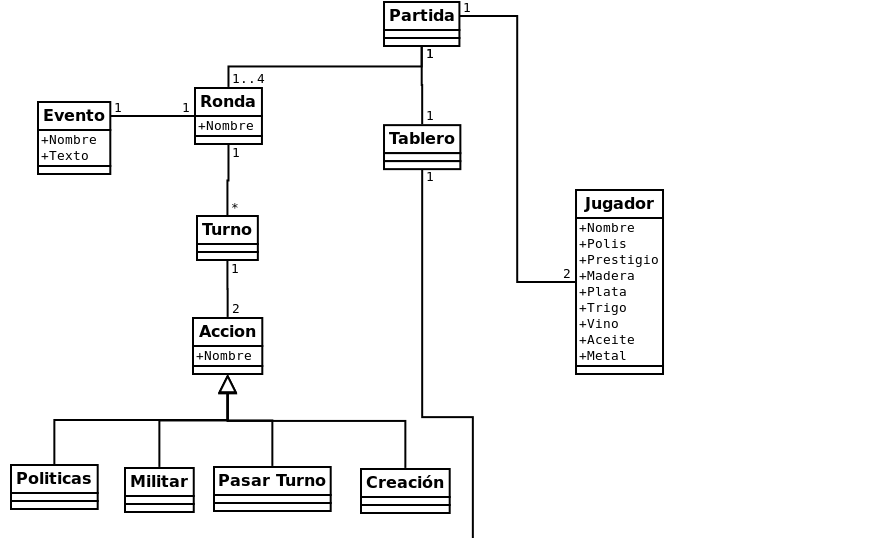
\includegraphics[width=500px]{analysis-uml/iteration2/part1.png}
			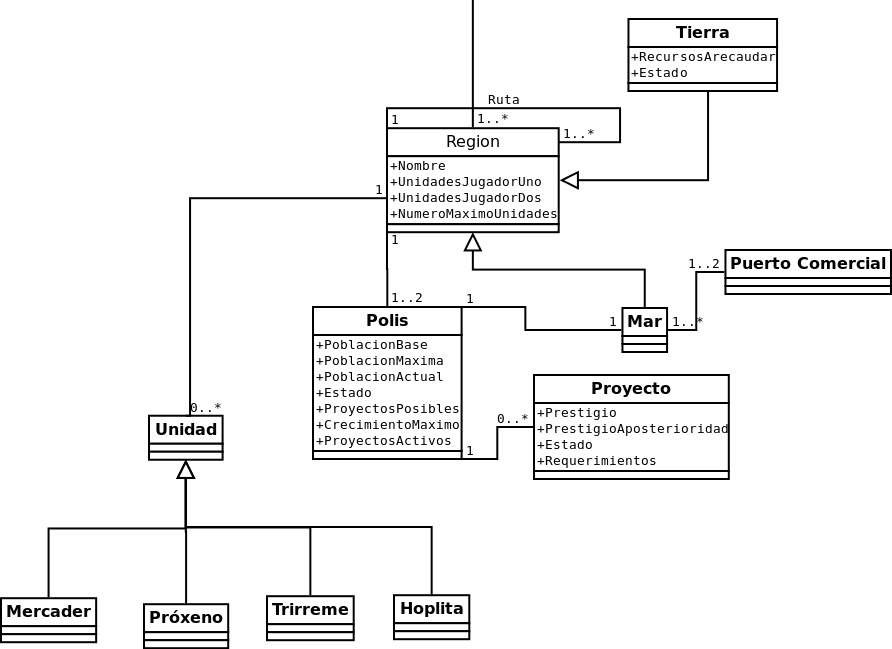
\includegraphics[width=500px]{analysis-uml/iteration2/part2.png}
		\end{center}
		
\chapter{Iteración 3}
	\section{Planificación Temporal}
		La primera entrega del proyecto será el día 7 de Octubre de 2010. Las siguientes entregas (2ª y 3ª Iteración) serán, respectivamente, los días 14 de Octubre y 11 de noviembre respectivamente.

	\section{Memorando técnico}
		En este tiempo se diseñó el diagrama UML de diseño del proyecto, se modificó el diagrama UML de análisis del proyecto, se realizó el diagrama de asignación de responsabilidades y se preparó el entorno técnico (Eclipse y Subversion) para el desarrollo del proyecto.
		
	\section{Seguimiento}
		\begin{tabular}{|c|c|c|c|}
			\hline
			Nombre & Tiempo dedicado acumulado & Puntuación & Puntuación acumulada\\
			\hline
			Samuel Navas Portillo & 30h & 6 & 16\\
			Juan Jesús Pérez Luna & 31h 30min & 8 & 18\\
			Manuel de los Santos Campos & 23h & 4 & 14\\
			María José Sancha Maya & 28h 30min & 4 & 14\\
			Ángel Martínez Olivares & 26h 30min & 4 & 14\\
			José Antonio Jiménez Carmona & 27h & 4 & 14\\
			\hline
		\end{tabular}

	\section{Diagrama UML de Análisis}
		\begin{center}
			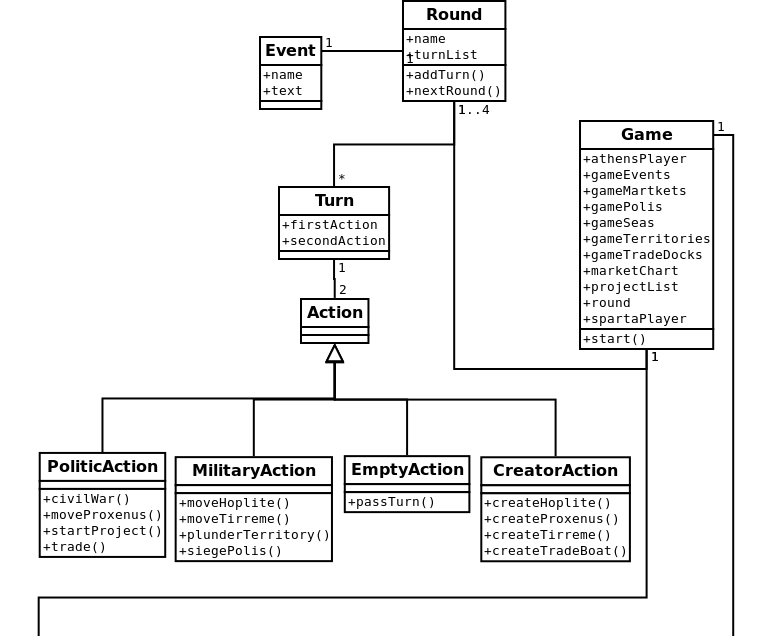
\includegraphics[width=500px]{analysis-uml/iteration3/part1.png}
			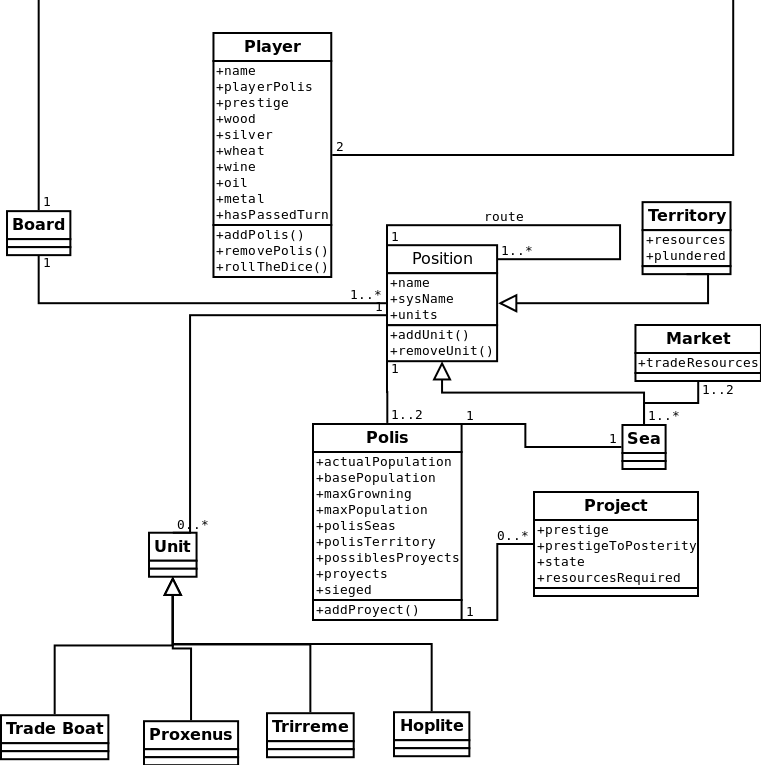
\includegraphics[width=500px]{analysis-uml/iteration3/part2.png}
		\end{center}

	\section{Asignación de Responsabilidades}
		\begin{center}
			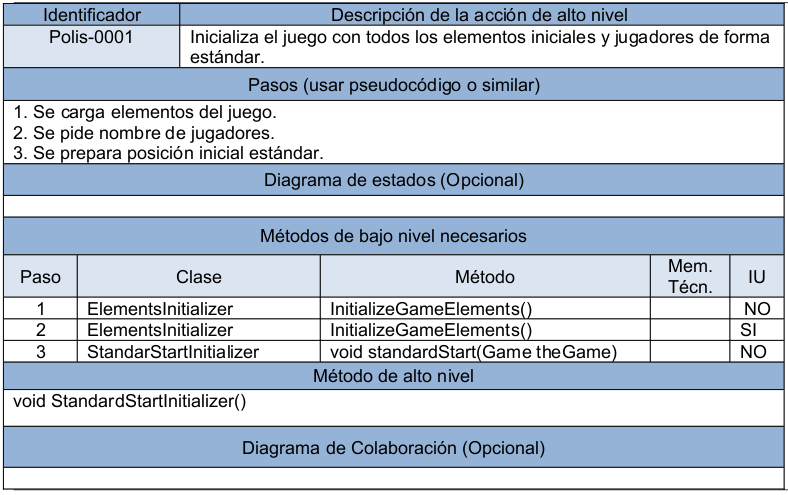
\includegraphics[width=500px]{responsabilities-allocation/iteration3/polis-0001.png}
			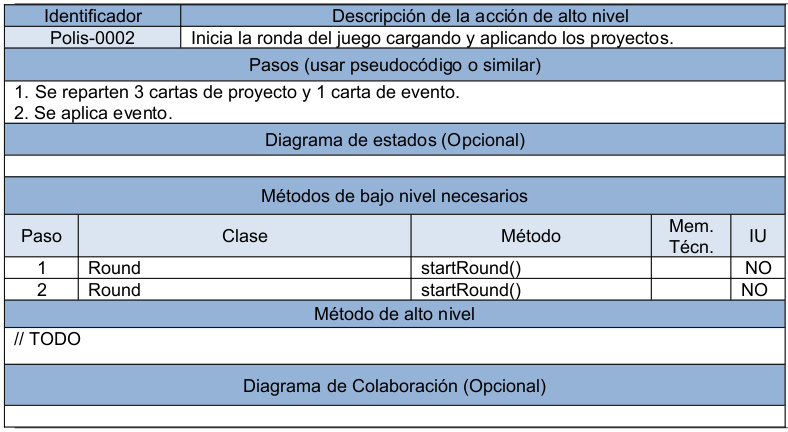
\includegraphics[width=500px]{responsabilities-allocation/iteration3/polis-0002.png}
			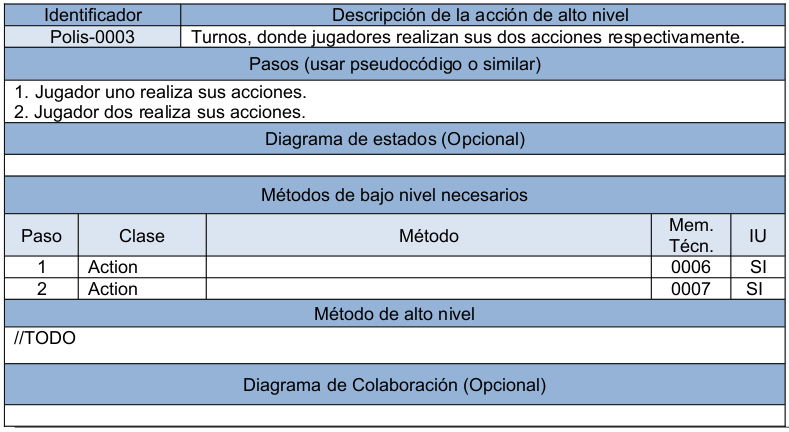
\includegraphics[width=500px]{responsabilities-allocation/iteration3/polis-0003.png}
			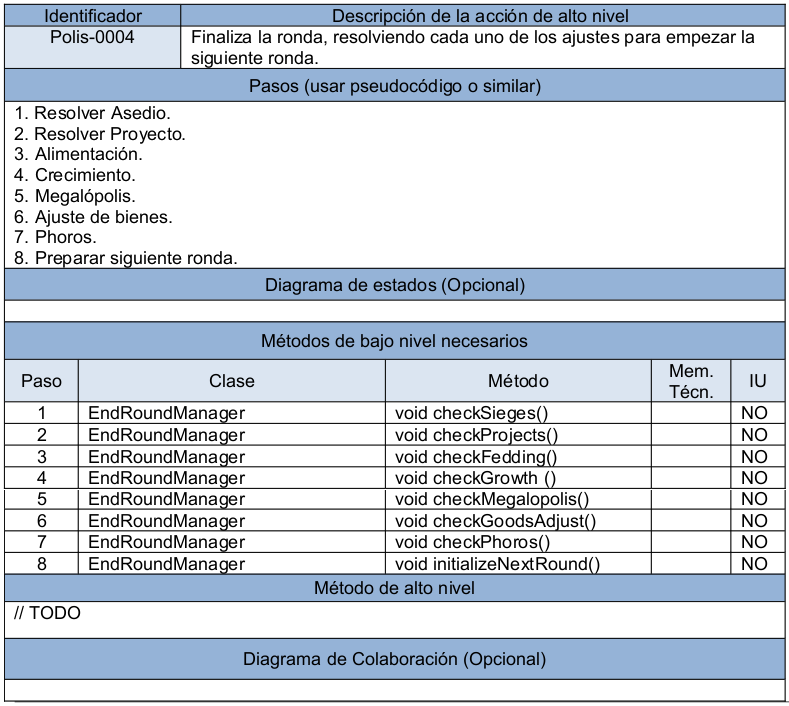
\includegraphics[width=500px]{responsabilities-allocation/iteration3/polis-0004.png}
			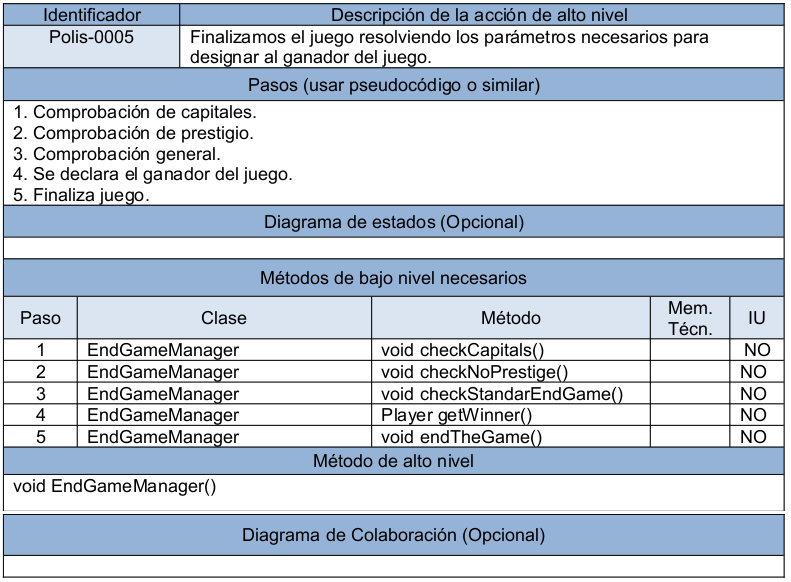
\includegraphics[width=500px]{responsabilities-allocation/iteration3/polis-0005.png}
			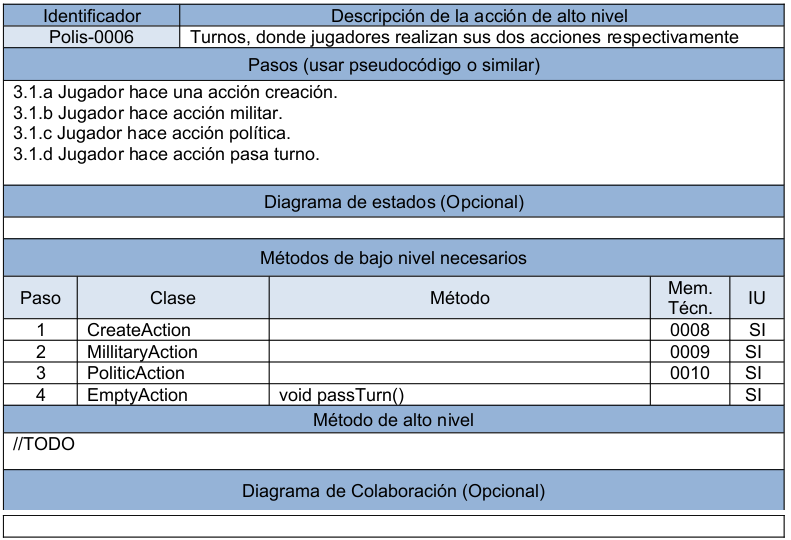
\includegraphics[width=500px]{responsabilities-allocation/iteration3/polis-0006.png}
			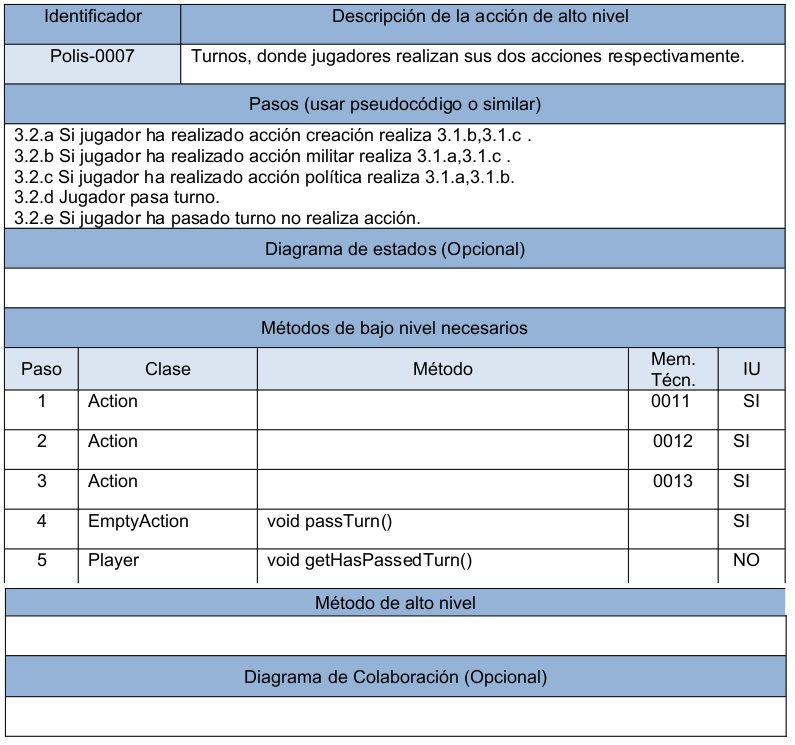
\includegraphics[width=500px]{responsabilities-allocation/iteration3/polis-0007.png}
			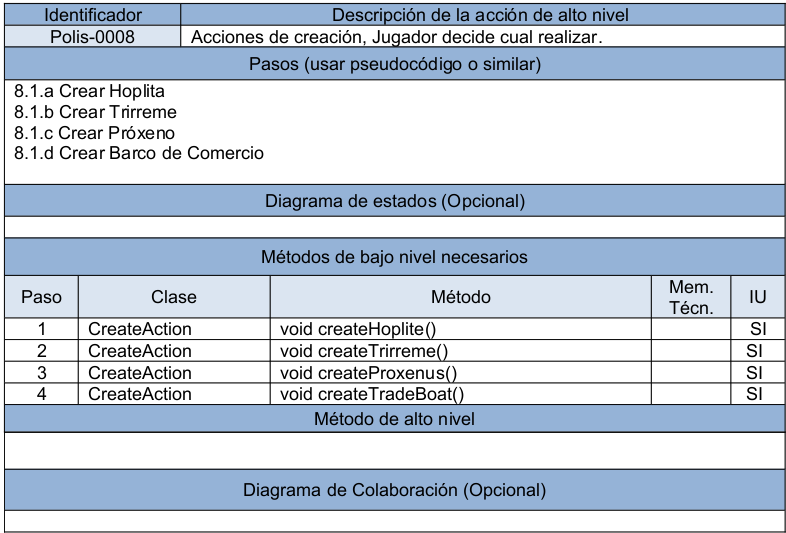
\includegraphics[width=500px]{responsabilities-allocation/iteration3/polis-0008.png}
			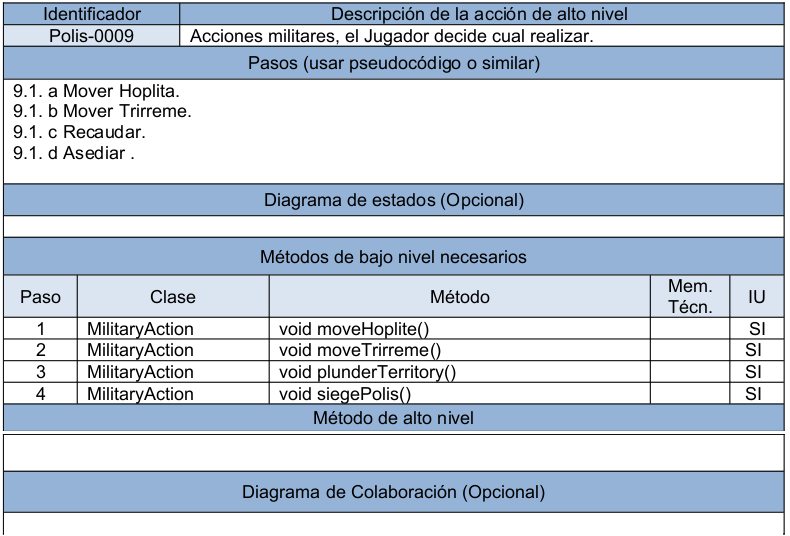
\includegraphics[width=500px]{responsabilities-allocation/iteration3/polis-0009.png}
			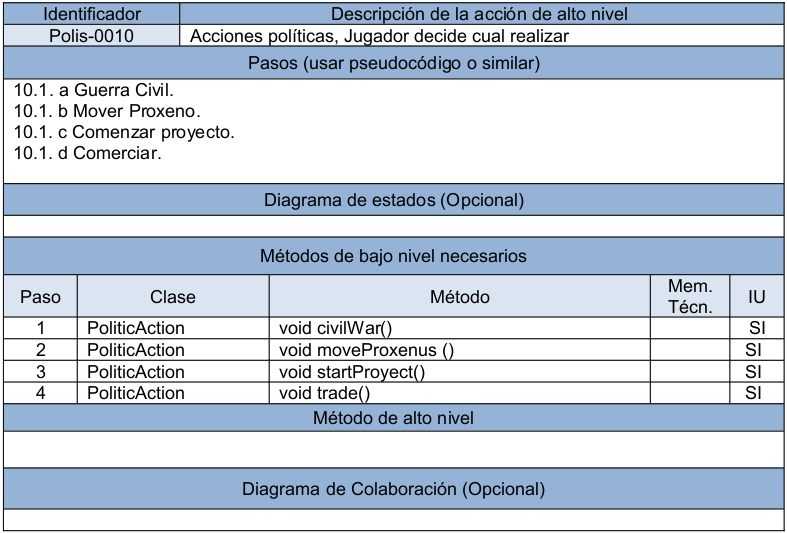
\includegraphics[width=500px]{responsabilities-allocation/iteration3/polis-0010.png}
			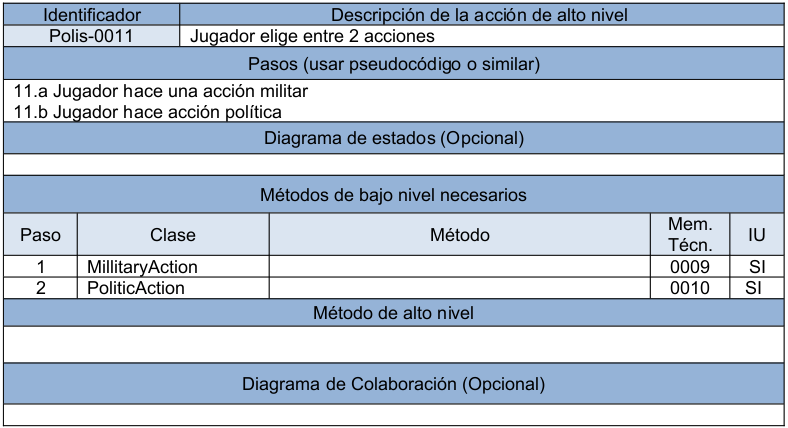
\includegraphics[width=500px]{responsabilities-allocation/iteration3/polis-0011.png}
			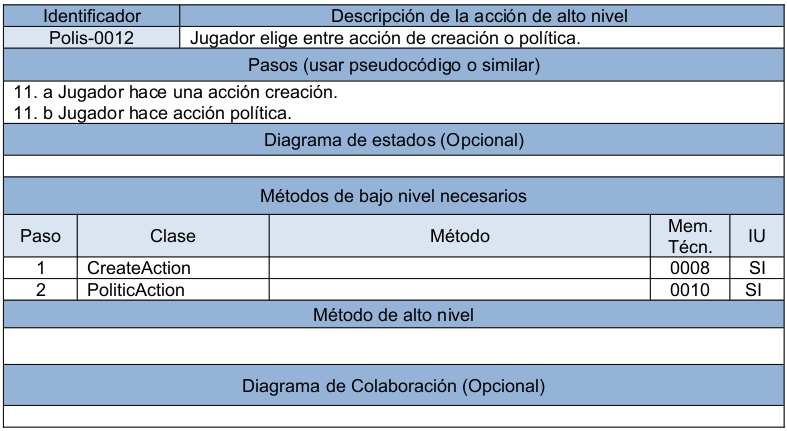
\includegraphics[width=500px]{responsabilities-allocation/iteration3/polis-0012.png}
			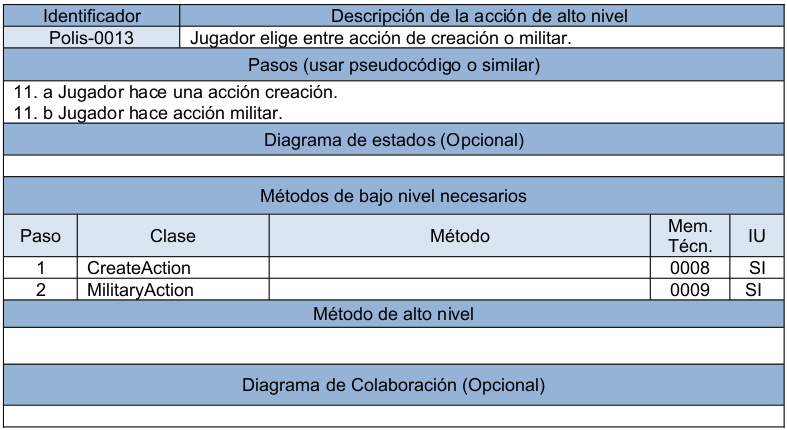
\includegraphics[width=500px]{responsabilities-allocation/iteration3/polis-0013.png}
		\end{center}

	\section{Diagrama UML de Diseño}
		\begin{center}
		    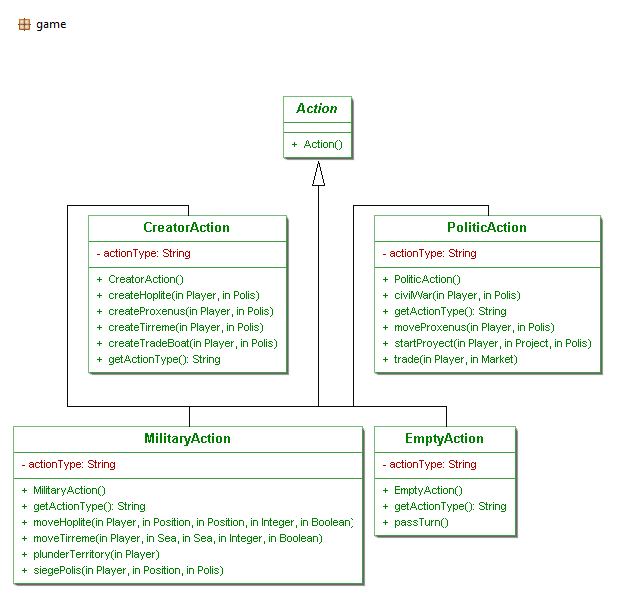
\includegraphics[width=500px]{design-uml/iteration3/game-actions.png}
		    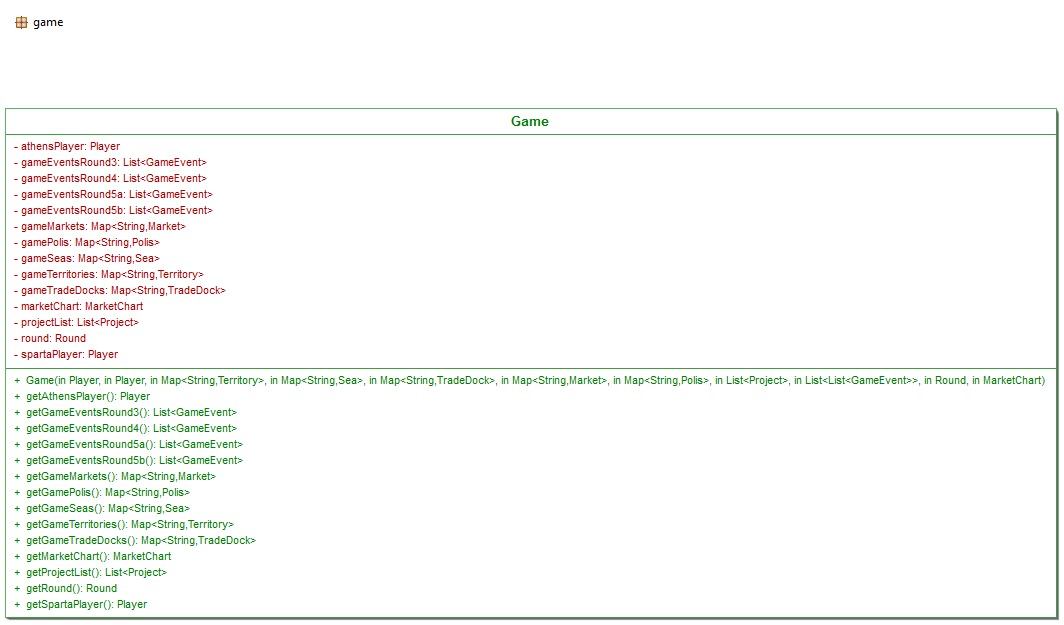
\includegraphics[width=500px]{design-uml/iteration3/game-game.png}
		    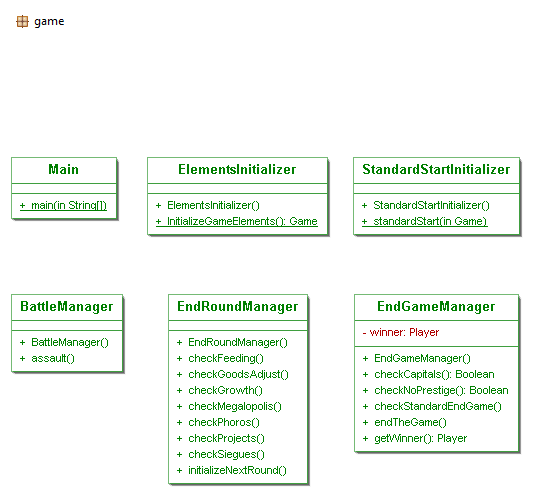
\includegraphics[width=500px]{design-uml/iteration3/game-main-managers.png}
		    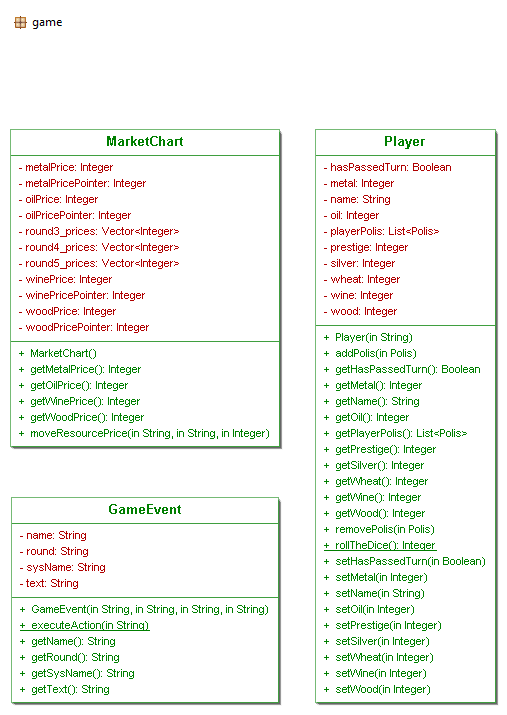
\includegraphics[width=500px]{design-uml/iteration3/game-martket-gameevent-player.png}
		    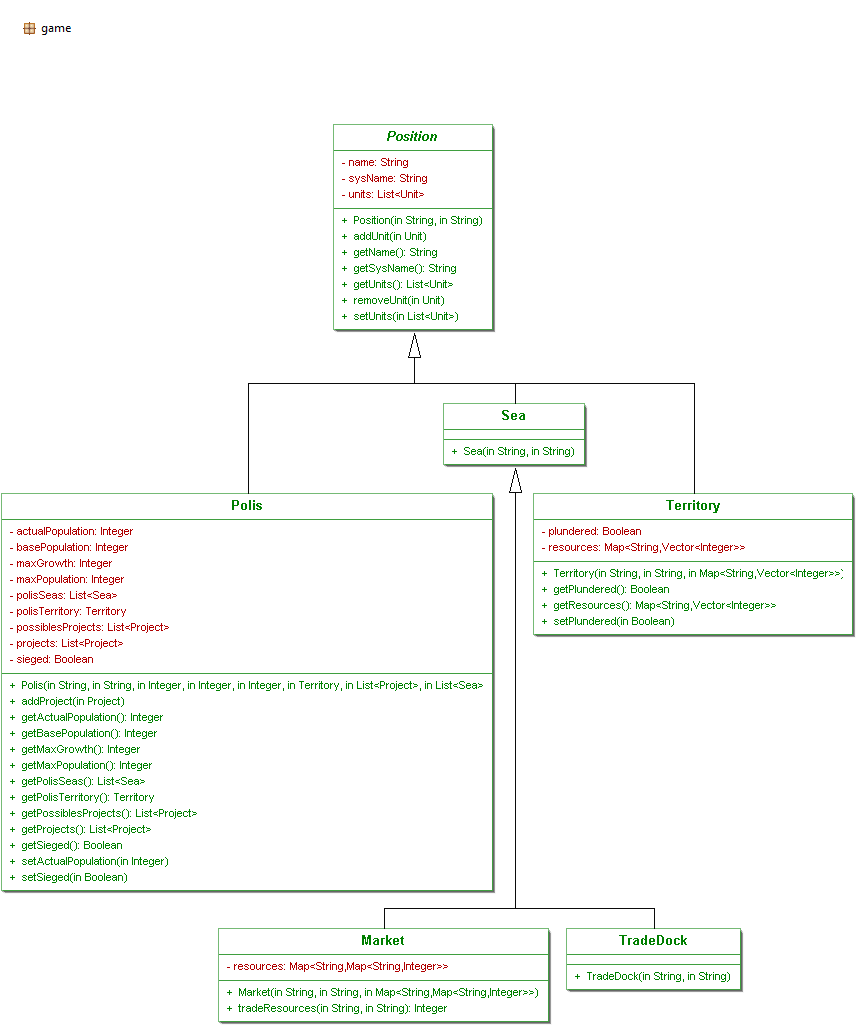
\includegraphics[width=500px]{design-uml/iteration3/game-positions.png}
		    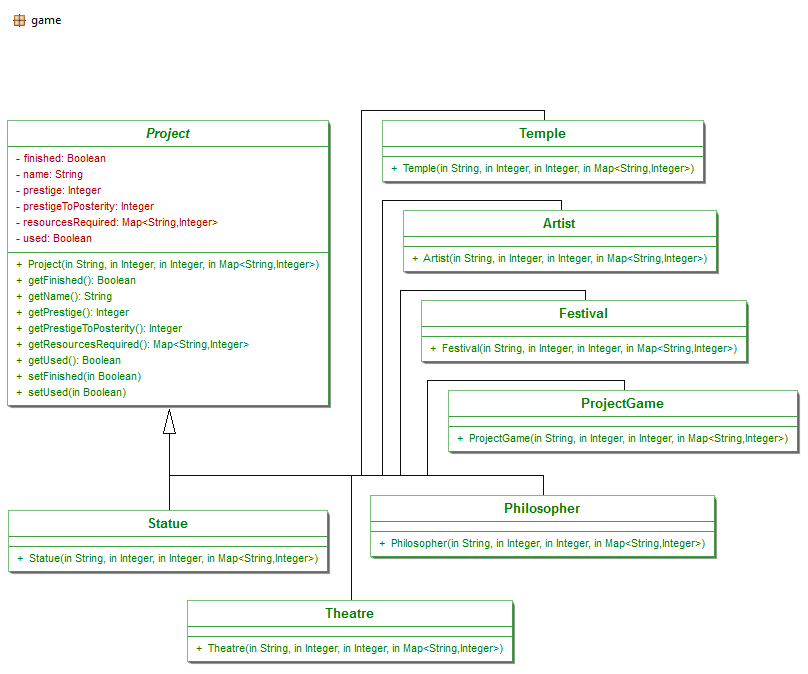
\includegraphics[width=500px]{design-uml/iteration3/game-projects.png}
		    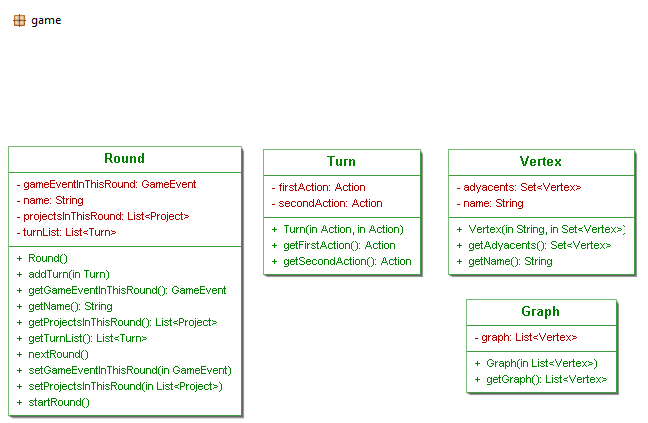
\includegraphics[width=500px]{design-uml/iteration3/game-round-turn-graph-vertex.png}
		    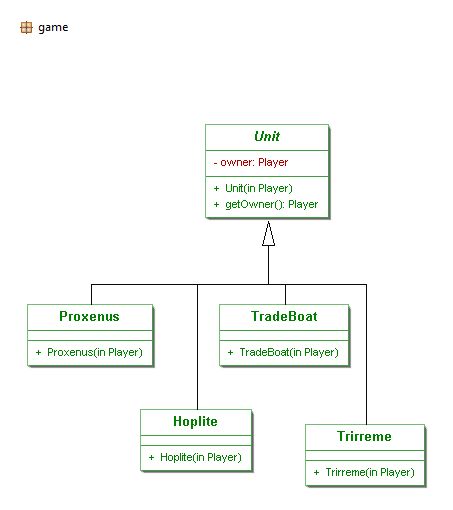
\includegraphics[width=500px]{design-uml/iteration3/game-units.png}
		    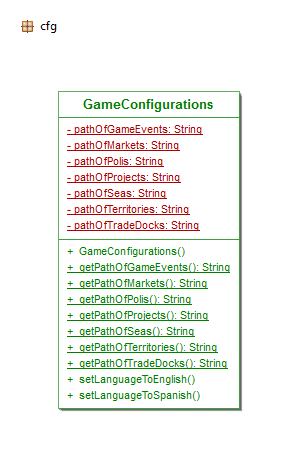
\includegraphics[width=500px]{design-uml/iteration3/package-cfg.png}
		    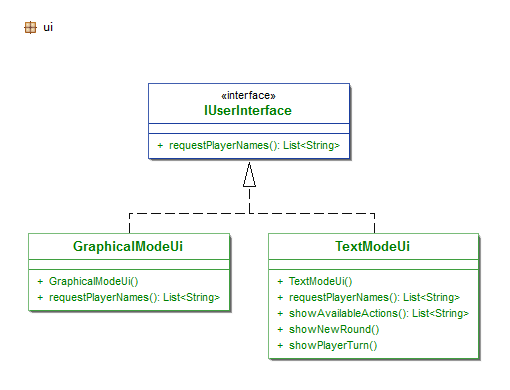
\includegraphics[width=500px]{design-uml/iteration3/package-ui.png}
		    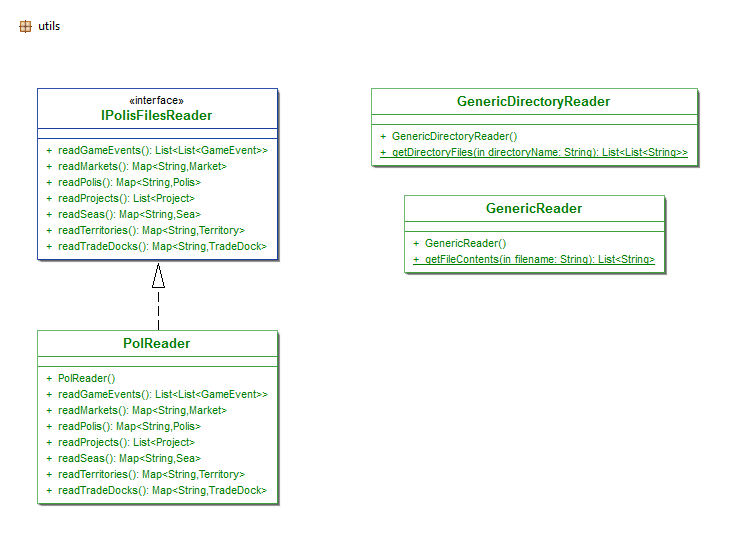
\includegraphics[width=500px]{design-uml/iteration3/package-utils.png}
		\end{center}
		
\chapter{Iteración 4}
	\section{Planificación Temporal}
		La entrega de la 4ª iteración será el día 3 de Diciembre.

	\section{Memorando técnico}
		En esta iteración se modificó el diagrama de asignación de responsabilidades y se implementó la arquitectura de código del proyecto y parte de sus clases y funciones.
		
	\section{Seguimiento}
		\begin{tabular}{|c|c|c|c|}
			\hline
			Nombre & Tiempo dedicado acumulado & Puntuación & Puntuación acumulada\\
			\hline
			Samuel Navas Portillo & 60h & 6 & 22\\
			Juan Jesús Pérez Luna & 61h 30min & 6 & 24\\
			Manuel de los Santos Campos & 38 & 5 & 19\\
			María José Sancha Maya & 37h 30min & 3 & 17\\
			Ángel Martínez Olivares & 38h 30min & 4 & 18\\
			José Antonio Jiménez Carmona & 42 & 6 & 20\\
			\hline
		\end{tabular}

	\section{Asignación de Responsabilidades}
		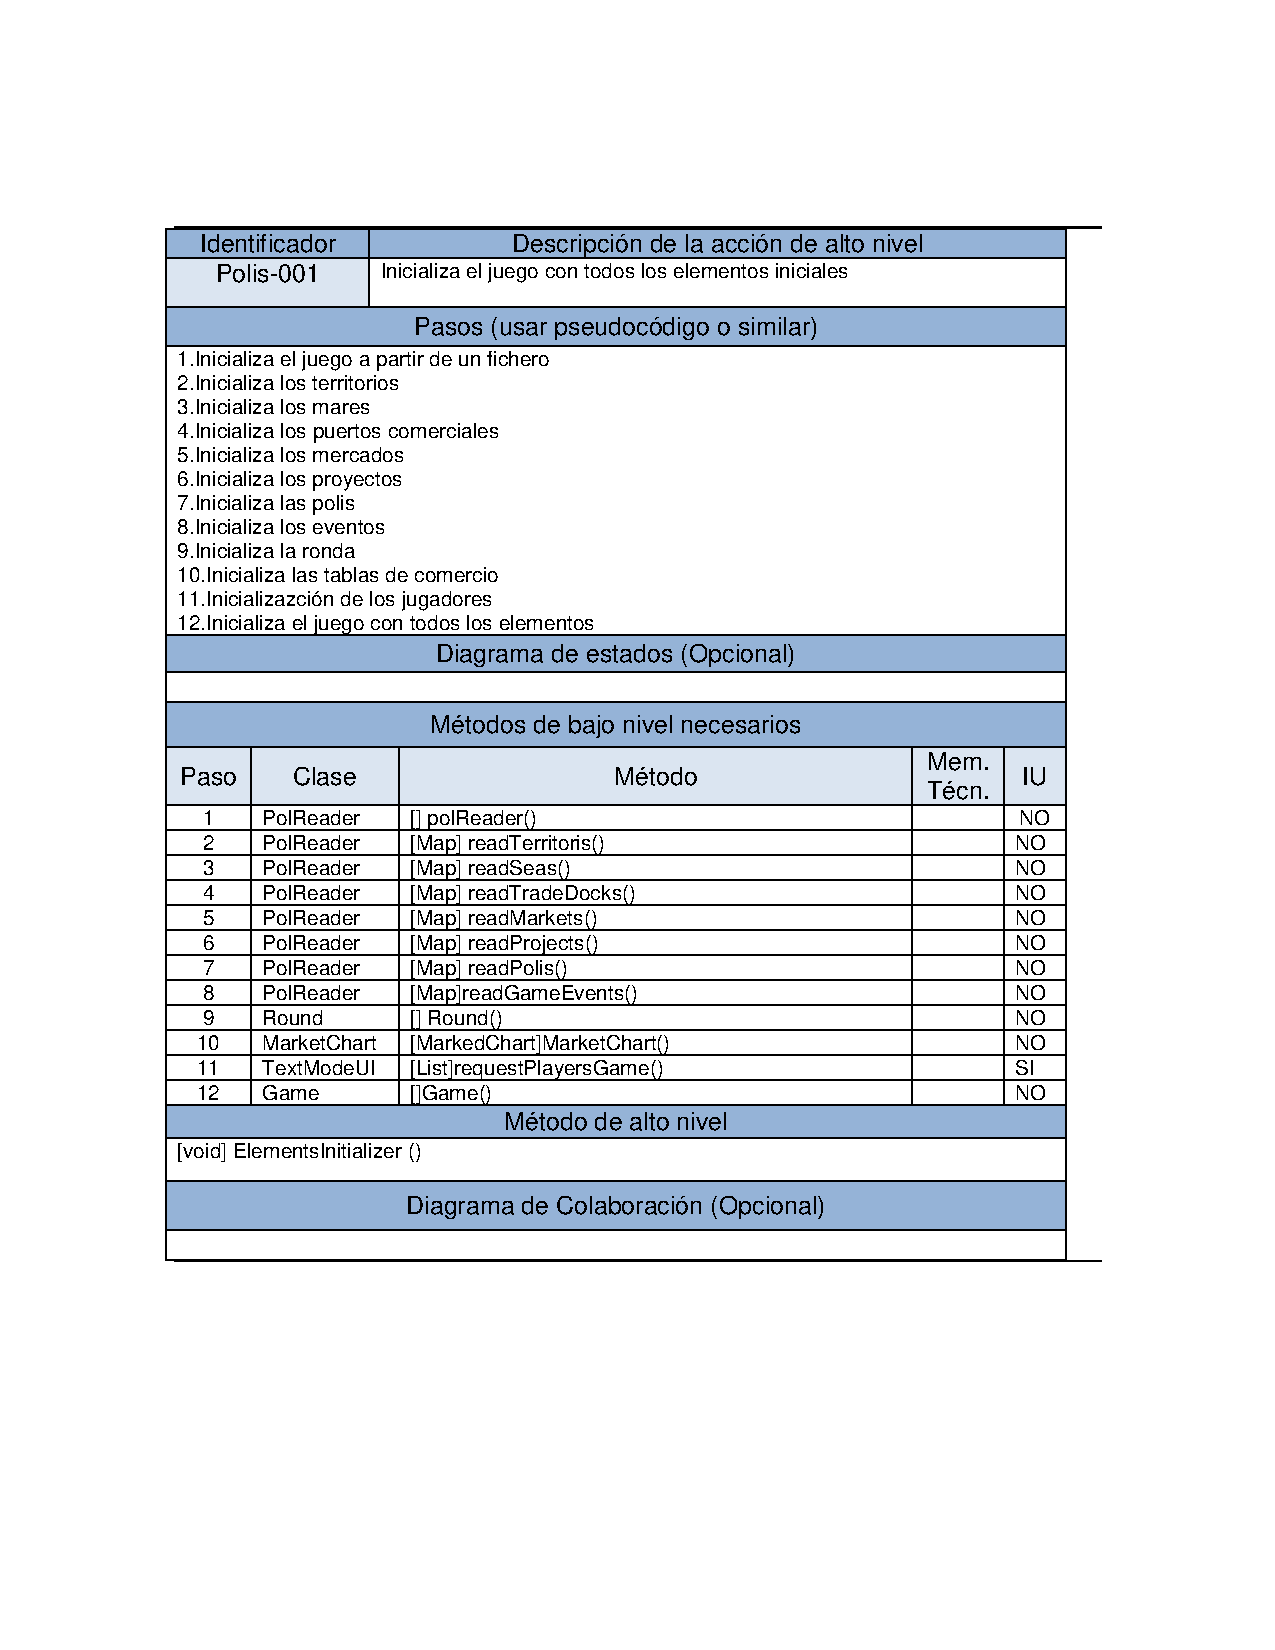
\includepdf[pages=-]{responsabilities-allocation/iteration4/dar.pdf}

\chapter{Iteración 5}
	\section{Planificación Temporal}
		La entrega de la 5ª iteración será el día 18 de Diciembre.
	
	\section{Memorando técnico}
		En esta etapa se ha completado el código del proyecto hasta terminarlo. Para la próxima etapa, queda pendiente la refactorización de algunas partes del código.
		
	\section{Seguimiento}
		\begin{tabular}{|c|c|c|c|}
			\hline
			Nombre & Tiempo dedicado acumulado & Puntuación & Puntuación acumulada\\
			\hline
			Samuel Navas Portillo & 90h & 6 & 28\\
			Juan Jesús Pérez Luna & 106h 30min & 6 & 30\\
			Manuel de los Santos Campos & 68 & 6 & 25\\
			María José Sancha Maya & 47h 30min & 1 & 18\\
			Ángel Martínez Olivares & 58h 30min & 5 & 23\\
			José Antonio Jiménez Carmona & 52 & 6 & 26\\
			\hline
		\end{tabular}
	
\chapter{Iteración 6}
	\section{Planificación Temporal}
		La entrega de la 6ª iteración será el día 11 de Enero.

	\section{Memorando técnico}
		Esta fase nos ha llevado a refactorizar el código del proyecto en una gran parte (especialmente la interfaz de usuario de consola), para hacer de éste un código más legible, más modular, con menos acoplamiento y más reutilizable. Esta iteración ha supuesto un esfuerzo bastante grande para el grupo porque ha sido necesario un análisis de todo el proyecto en profundidad, ya que no era trivial determinar qué partes del código había que cambiar.
		
	\section{Seguimiento}
		\begin{tabular}{|c|c|c|c|}
			\hline
			Nombre & Tiempo dedicado acumulado & Puntuación & Puntuación acumulada\\
			\hline
			Samuel Navas Portillo & 126 & 10 & 38\\
			Juan Jesús Pérez Luna & 136h 30min & 8 & 38\\
			Manuel de los Santos Campos & 69 & 1 & 26\\
			María José Sancha Maya & 48h 30min & 1 & 19\\
			Ángel Martínez Olivares & 59h 30min & 1 & 24\\
			José Antonio Jiménez Carmona & 82 & 9 & 35\\
			\hline
		\end{tabular}

\chapter{Iteración 7}
	\section{Planificación Temporal}
		La entrega de la 7ª iteración será el día 19 de Enero.
	
	\section{Diagrama UML de diseño}
	
	\section{Asignación de responsabilidades}
		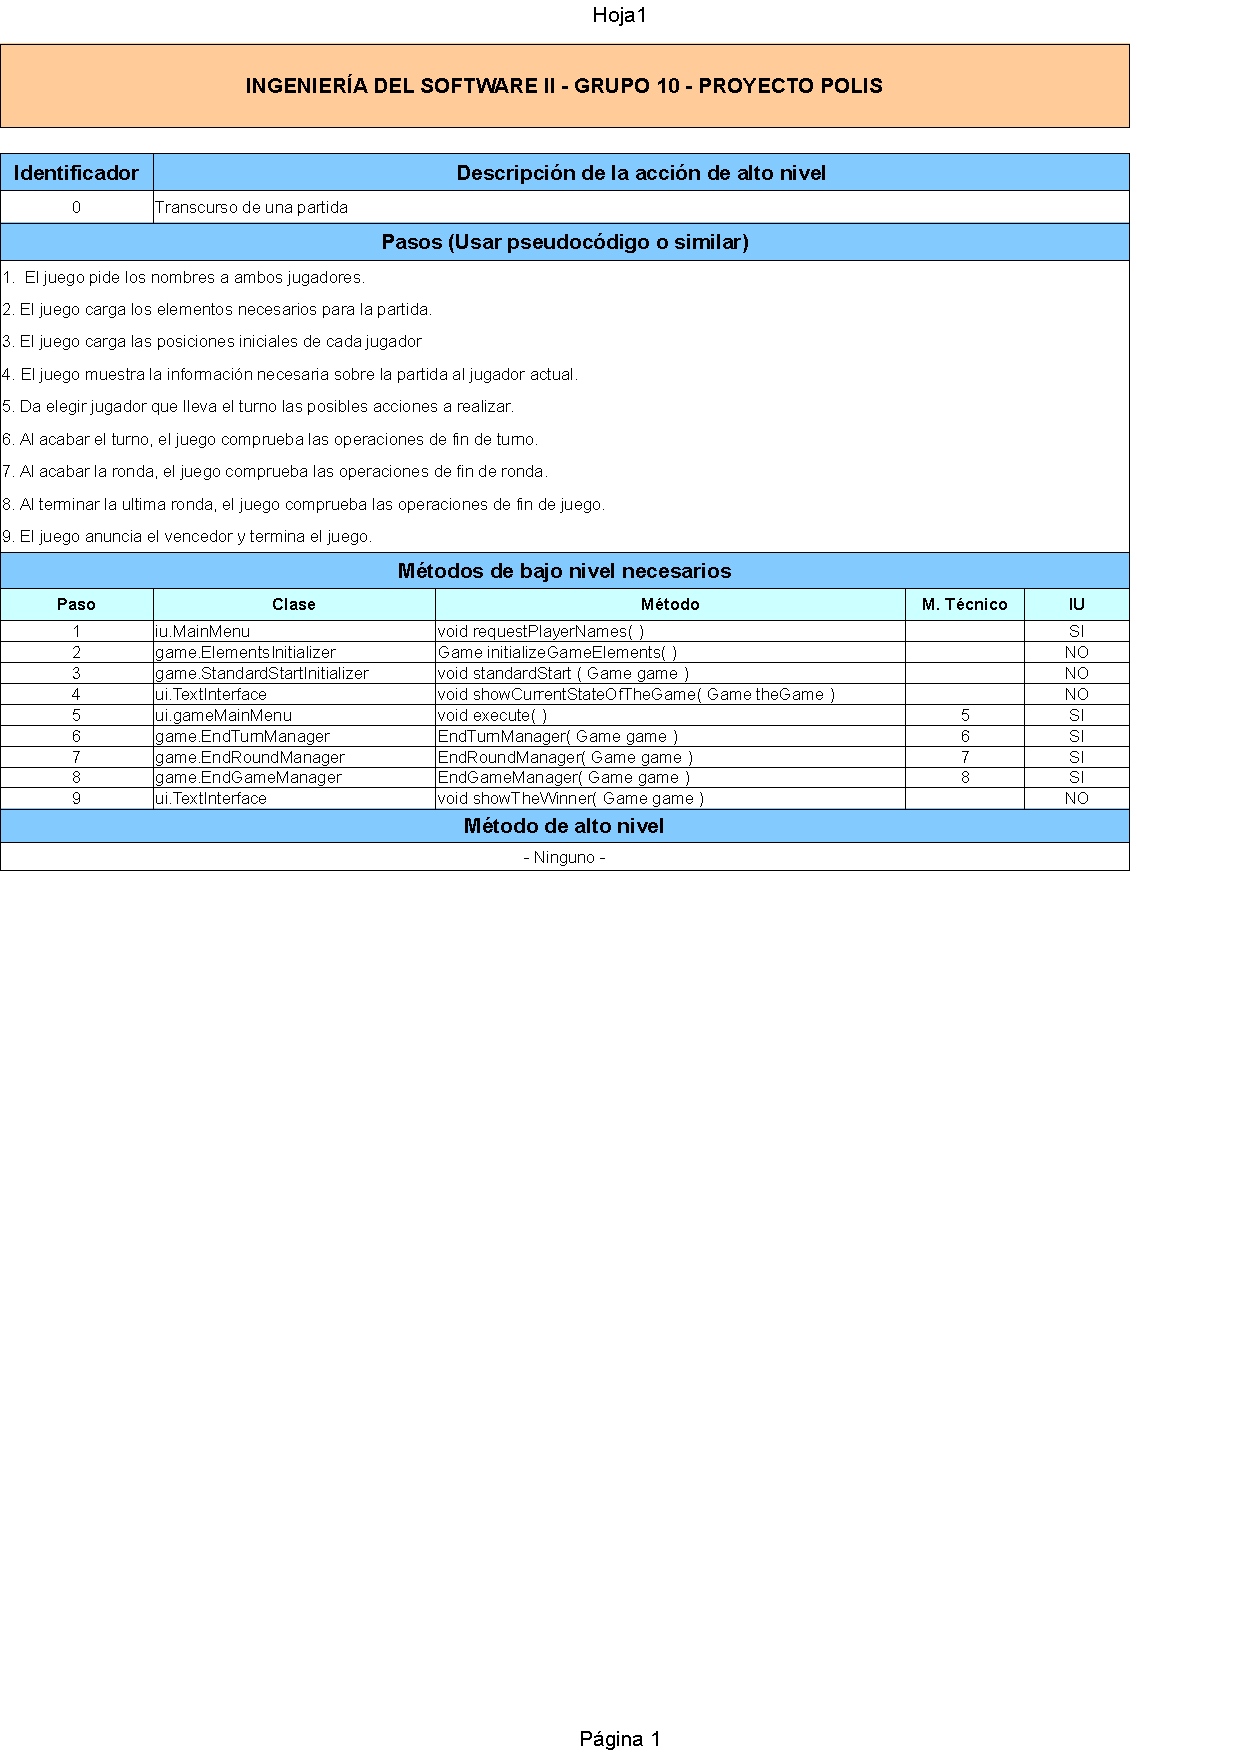
\includepdf[pages=-]{responsabilities-allocation/iteration7/IT7-00.pdf}
		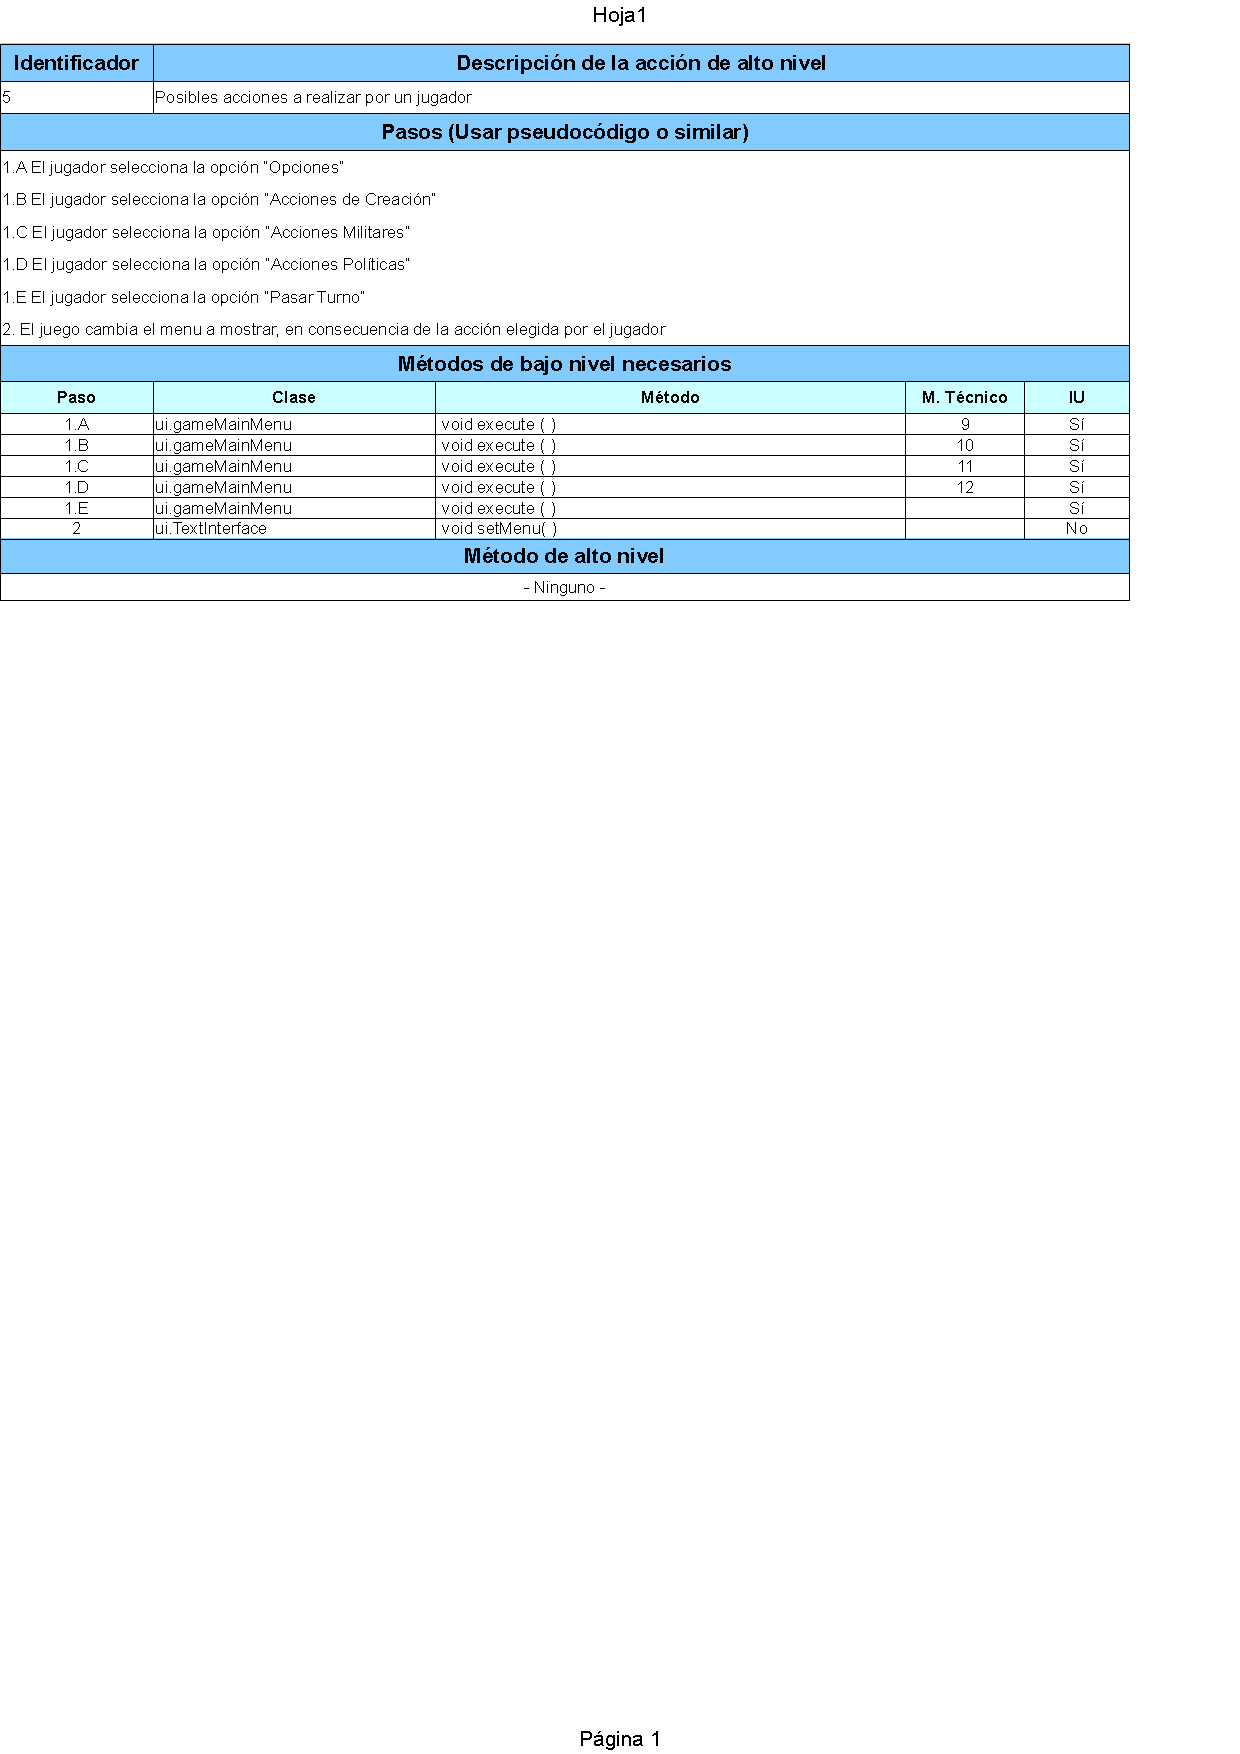
\includepdf[pages=-]{responsabilities-allocation/iteration7/IT7-05.pdf}
		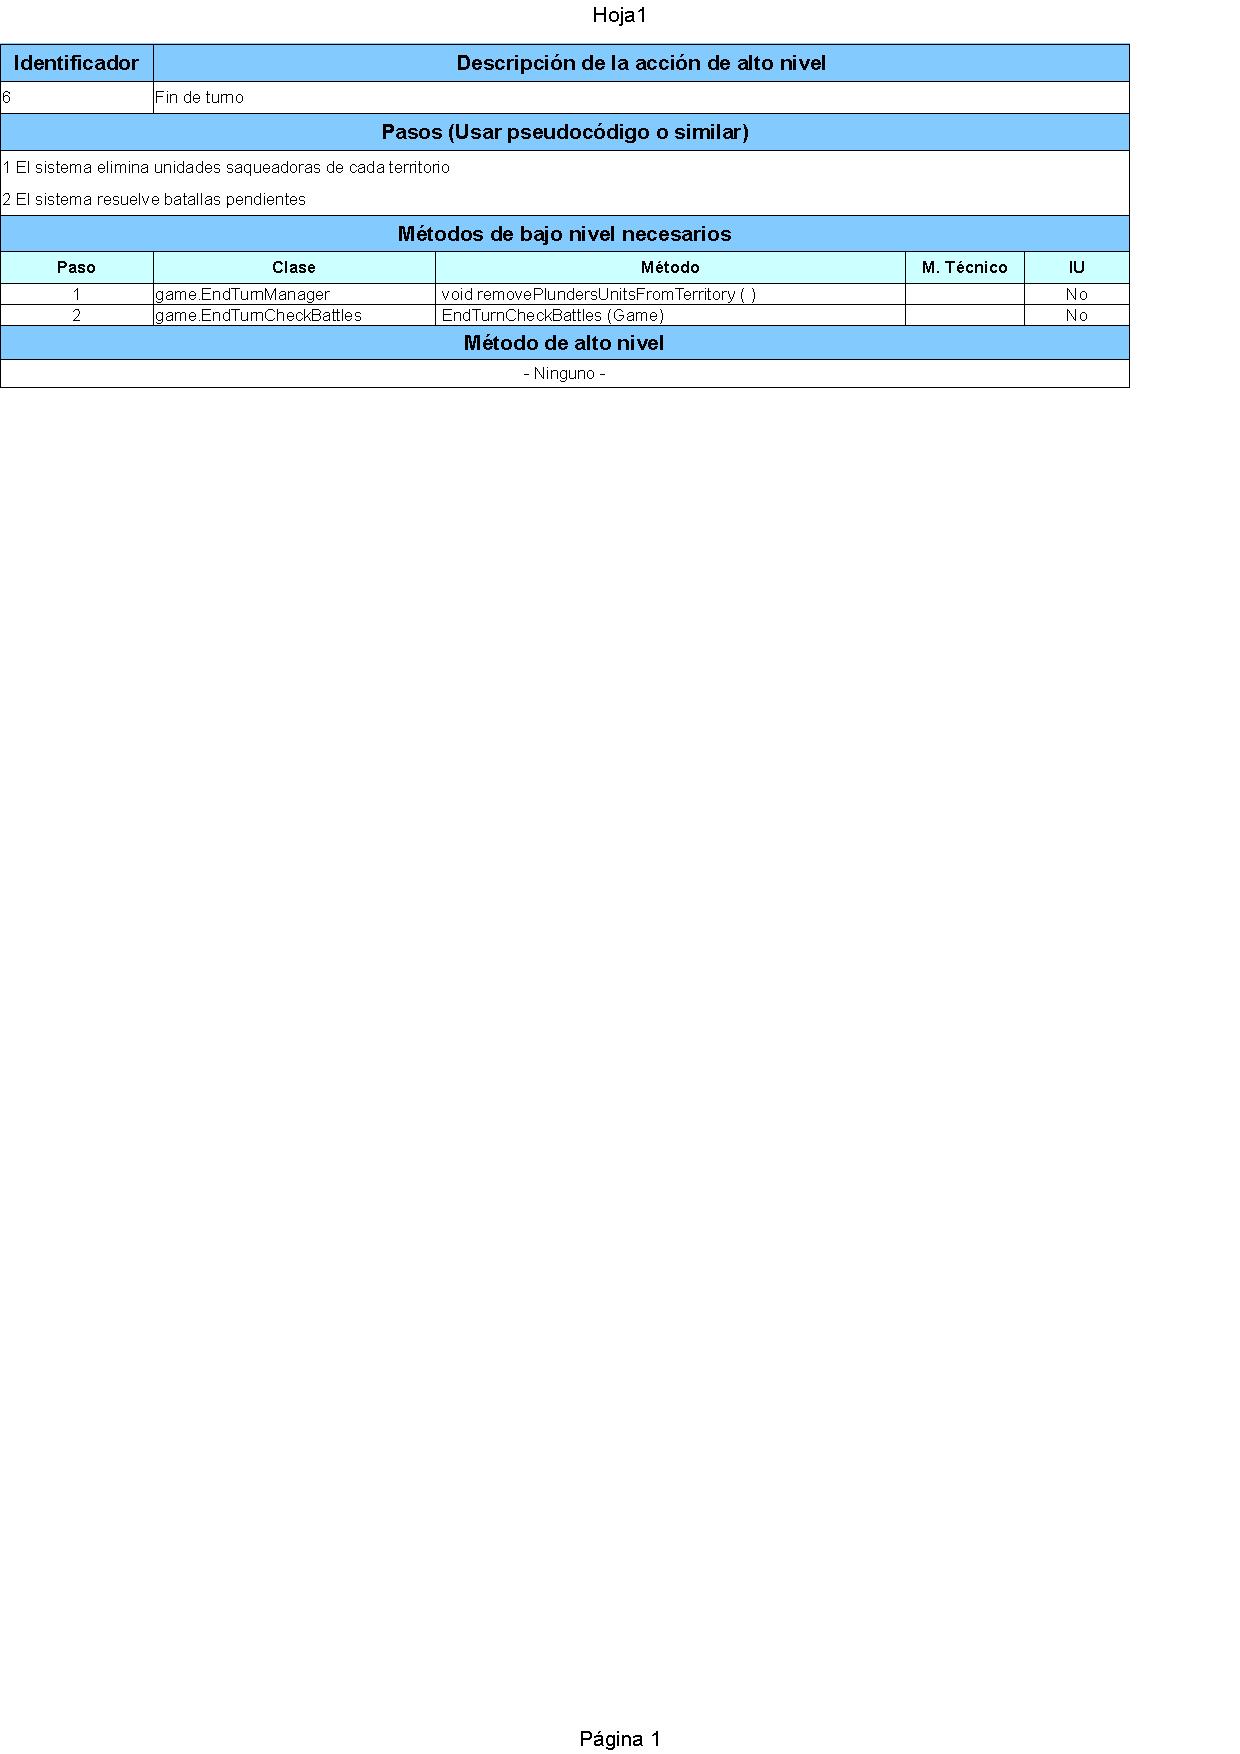
\includepdf[pages=-]{responsabilities-allocation/iteration7/IT7-06.pdf}
		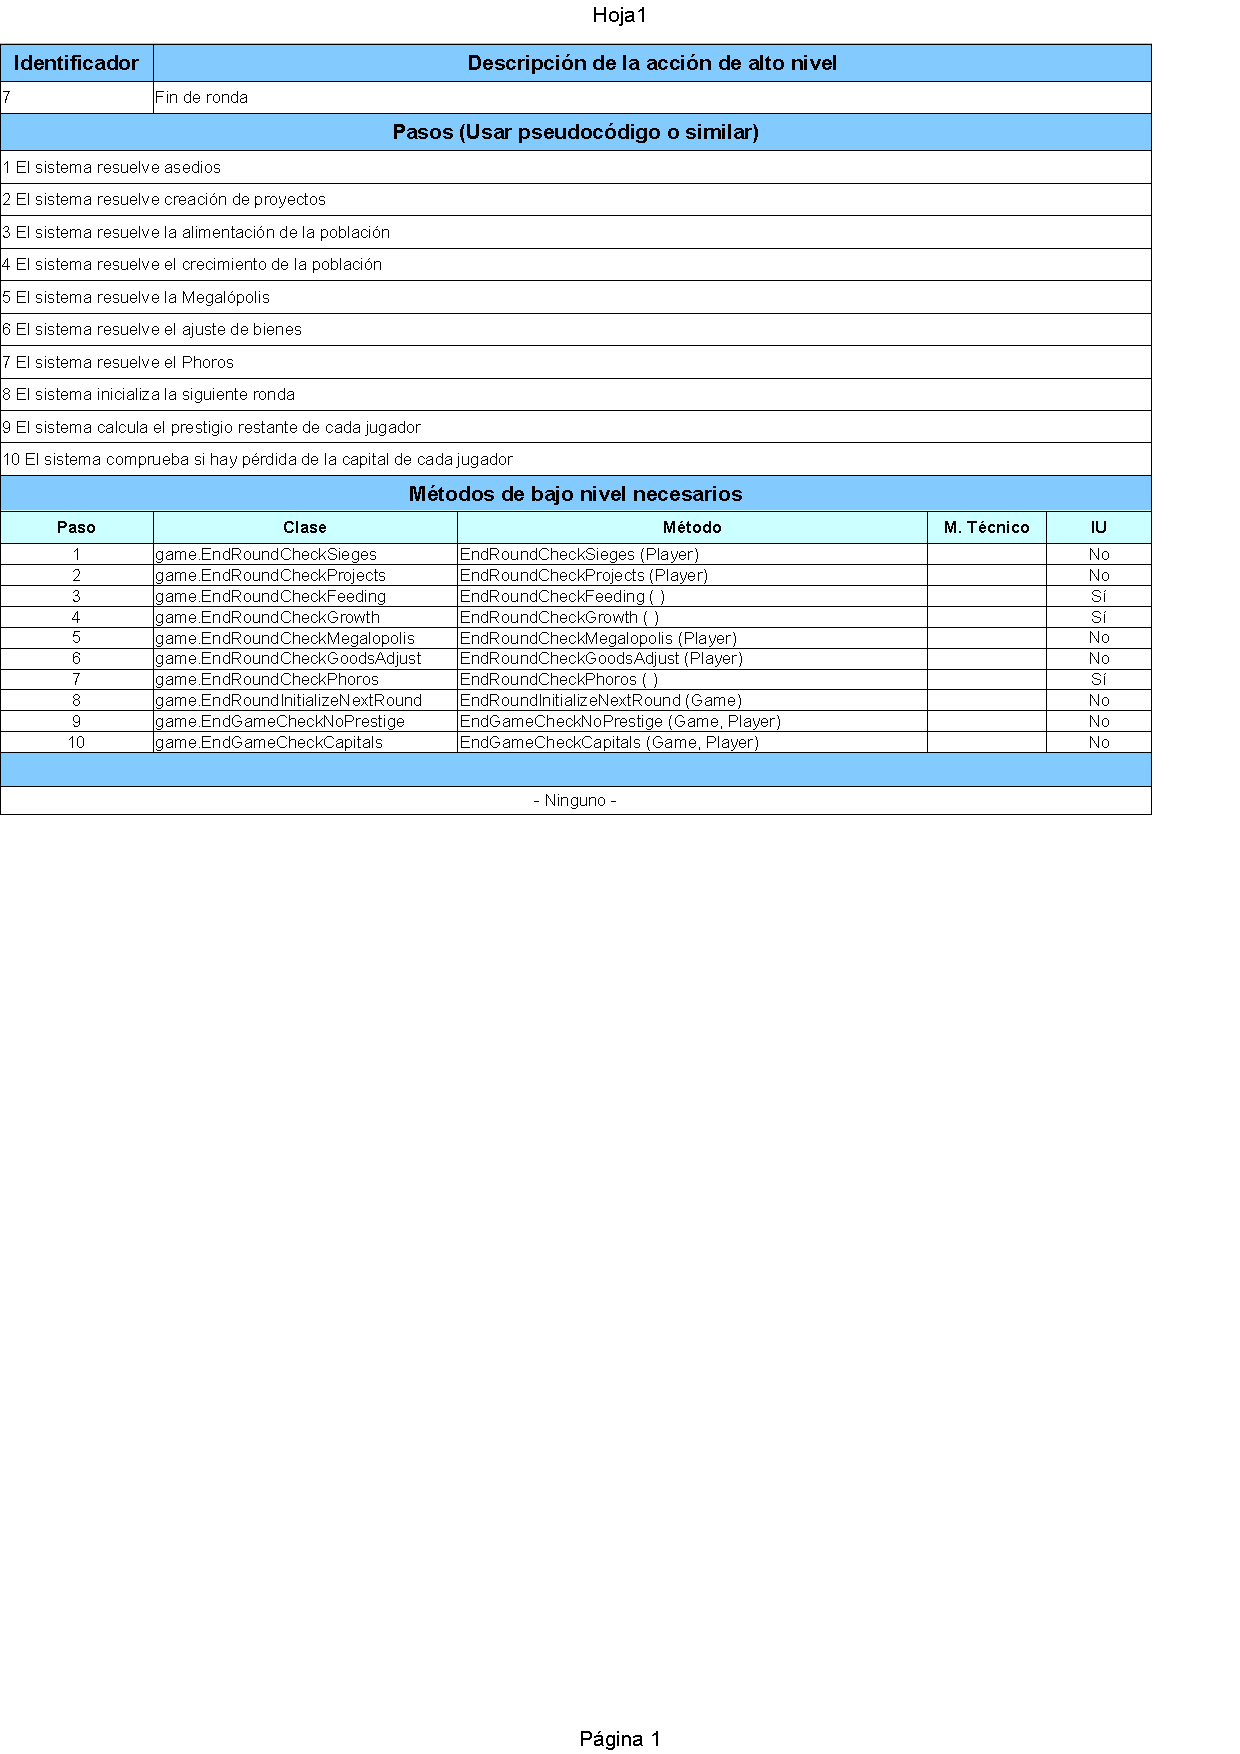
\includepdf[pages=-]{responsabilities-allocation/iteration7/IT7-07.pdf}
		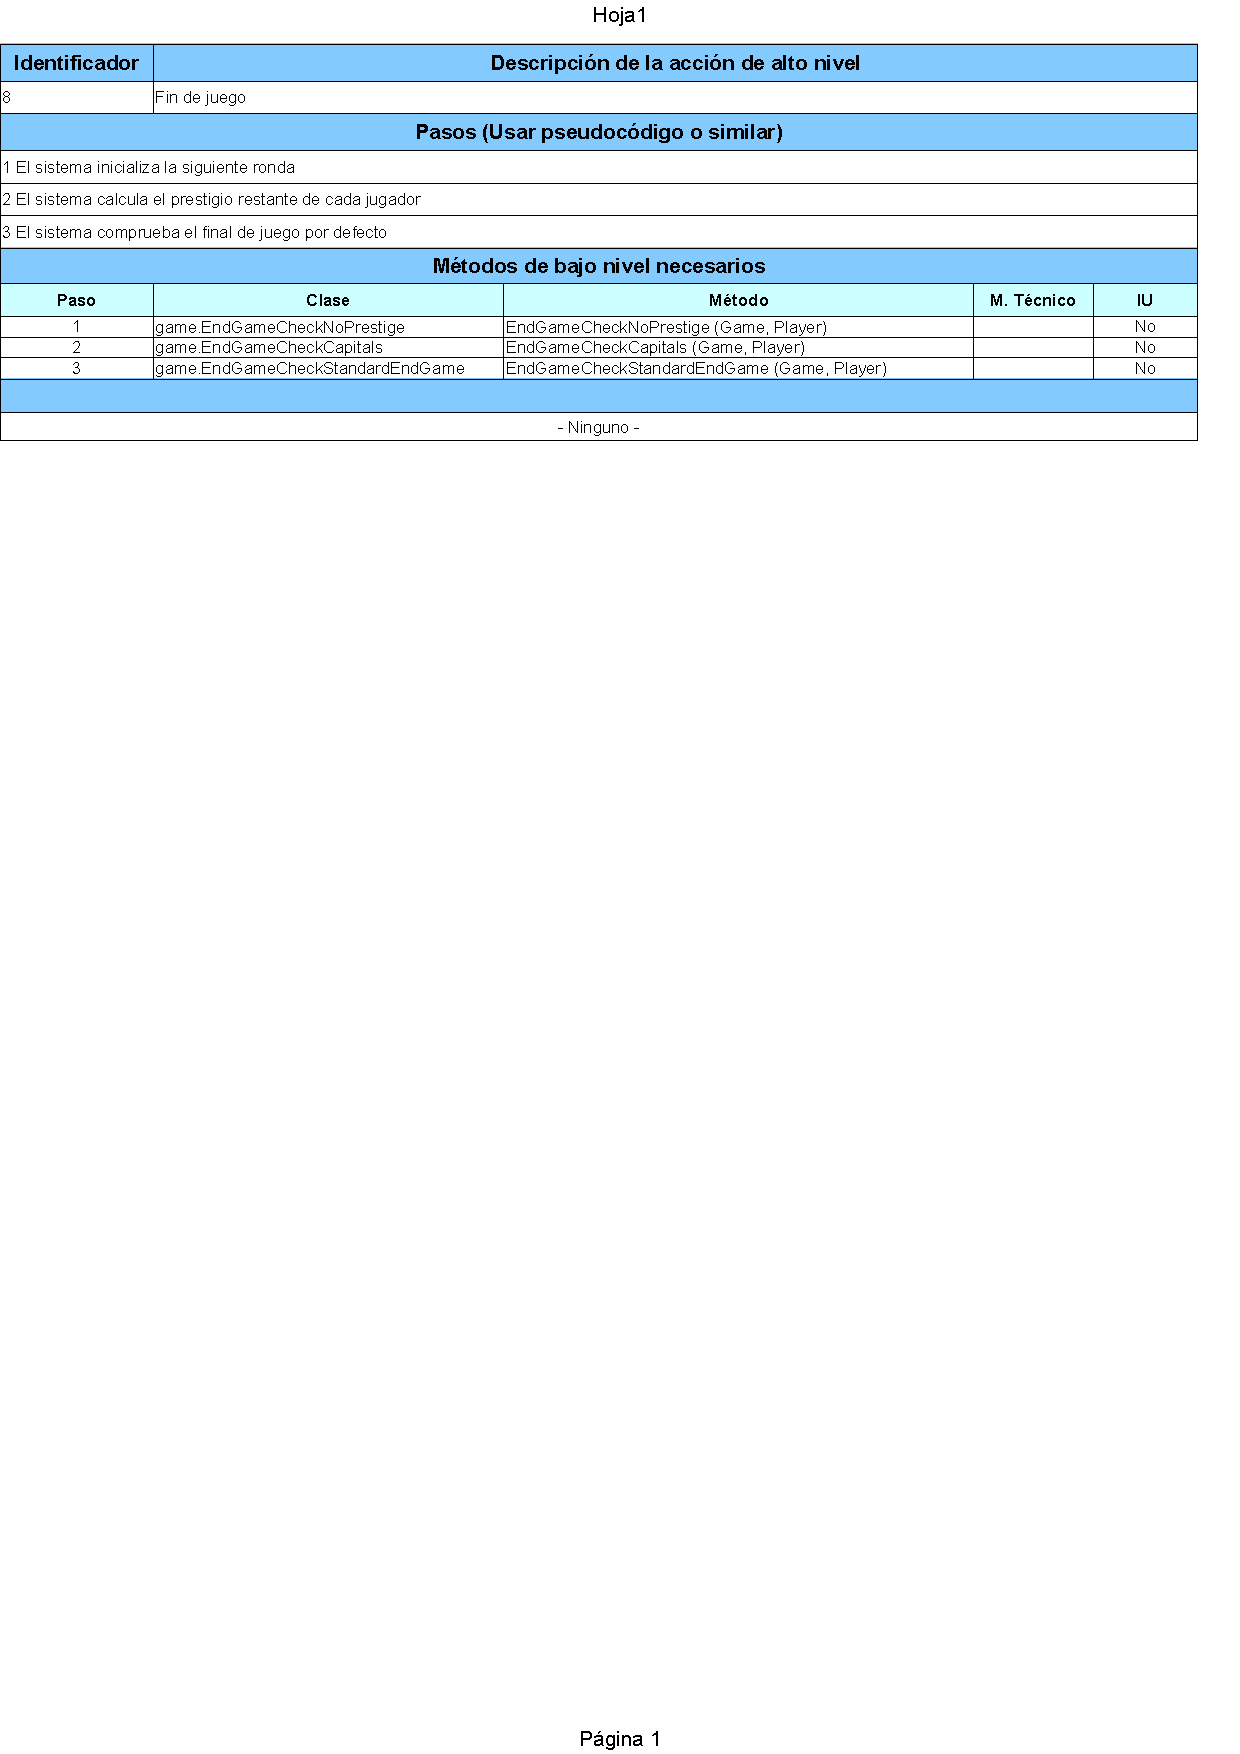
\includepdf[pages=-]{responsabilities-allocation/iteration7/IT7-08.pdf}
		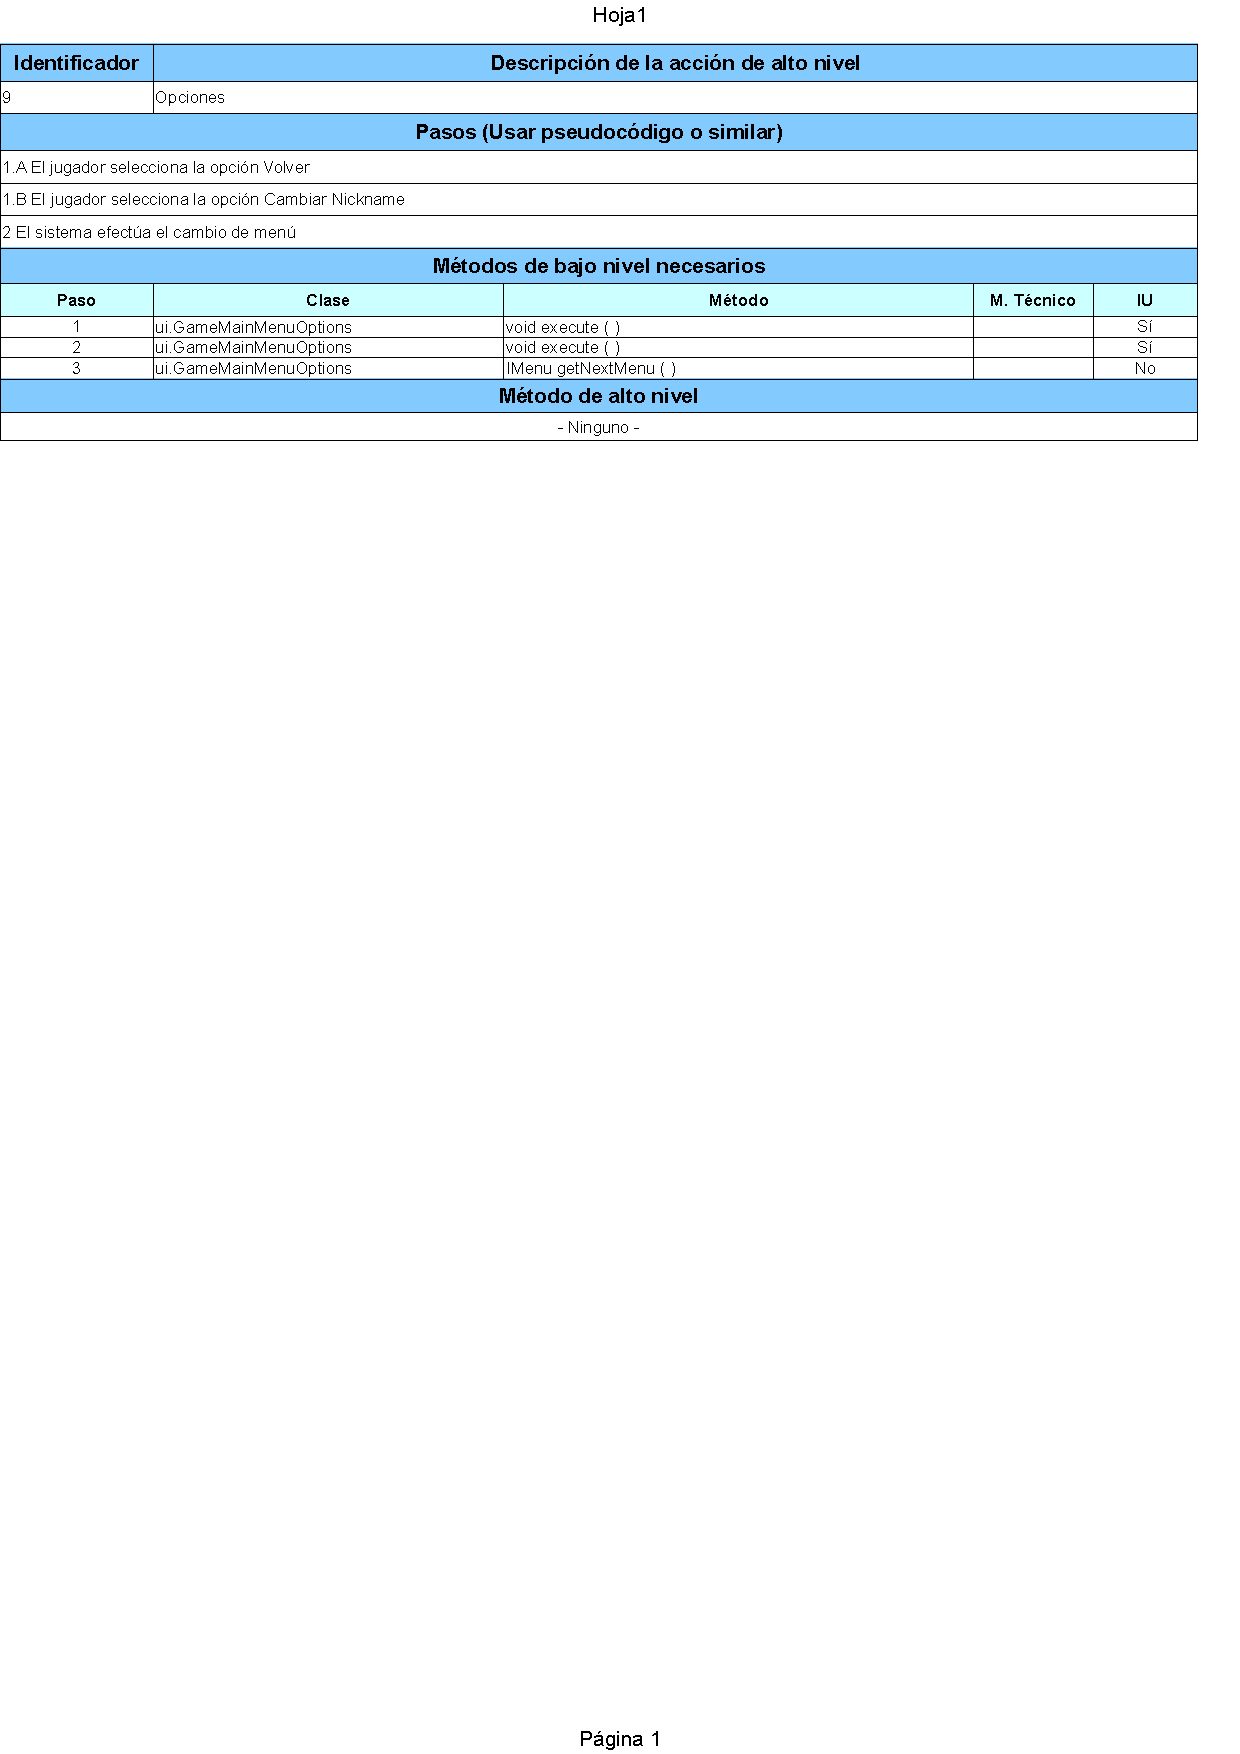
\includepdf[pages=-]{responsabilities-allocation/iteration7/IT7-09.pdf}
		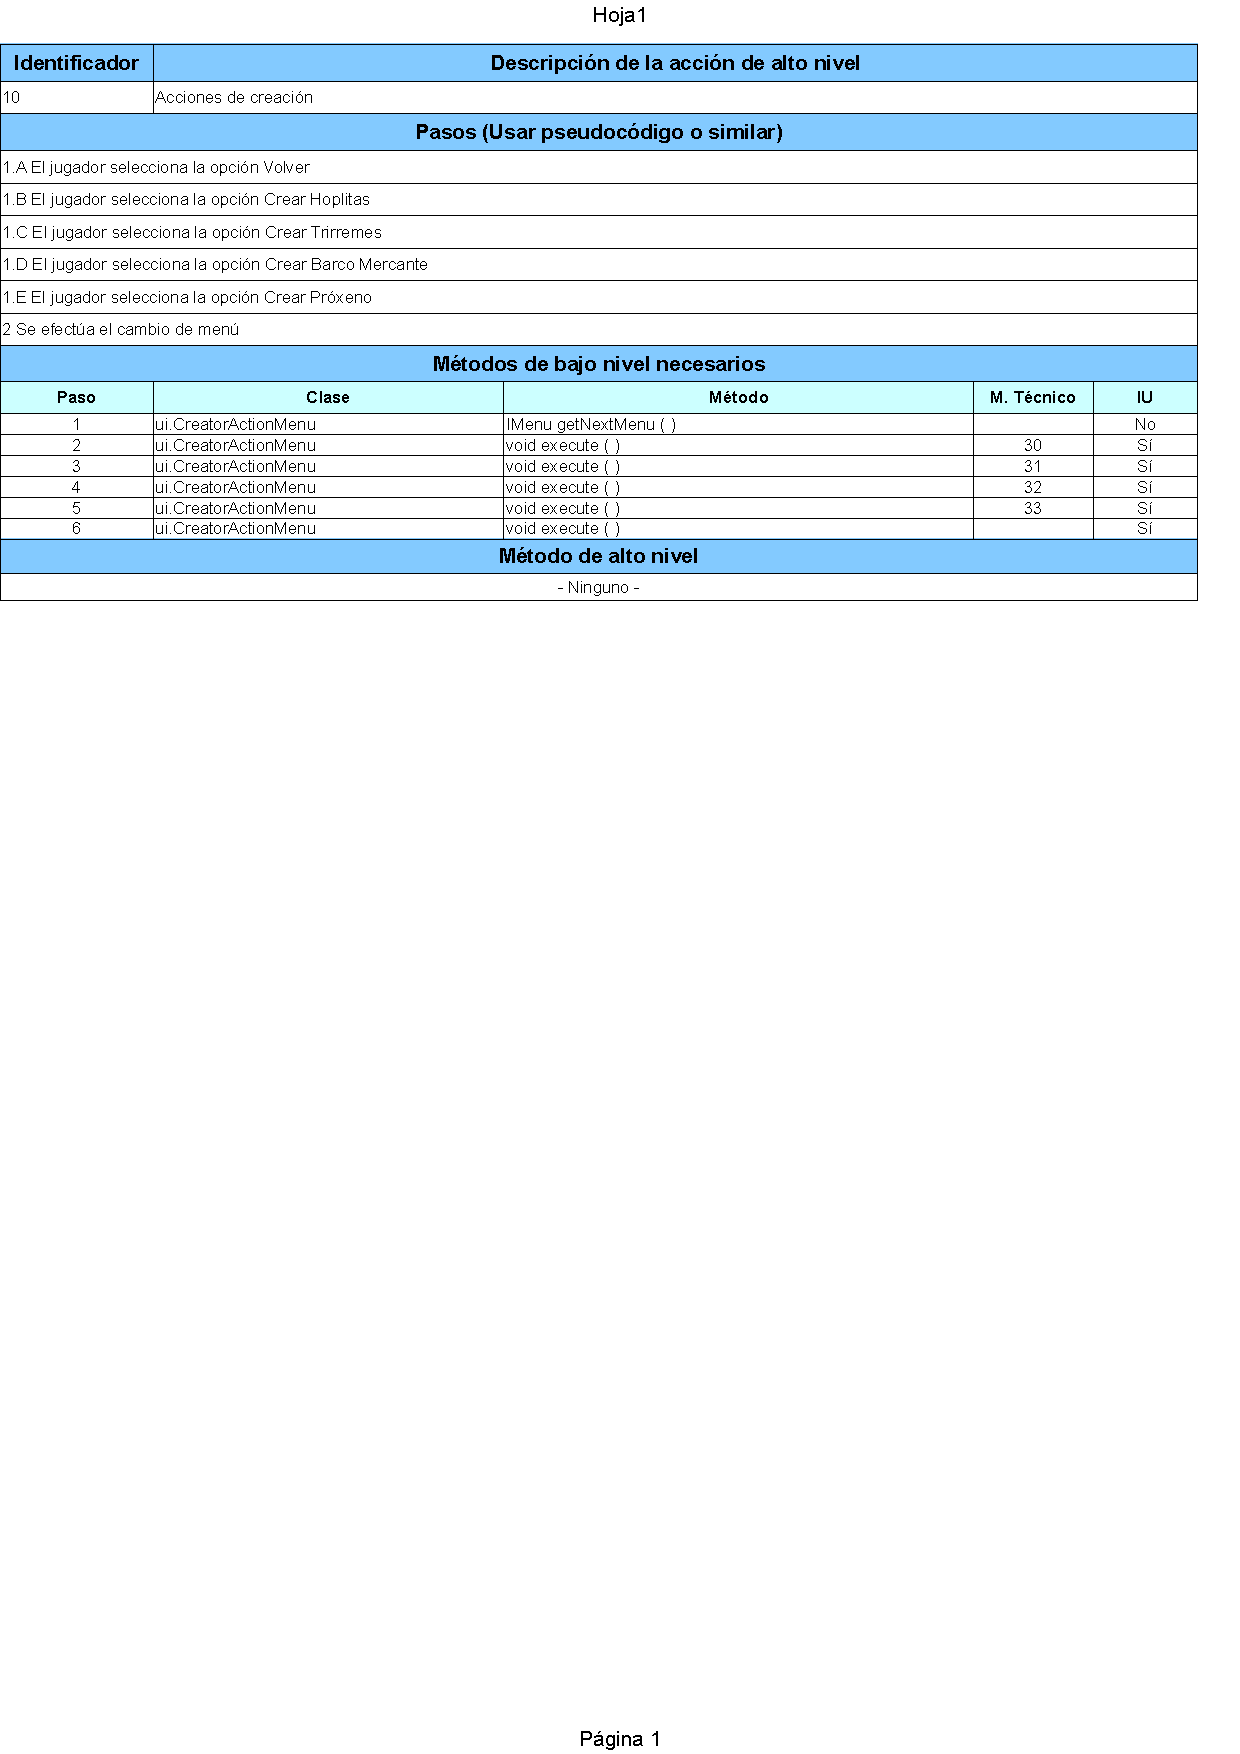
\includepdf[pages=-]{responsabilities-allocation/iteration7/IT7-10.pdf}
		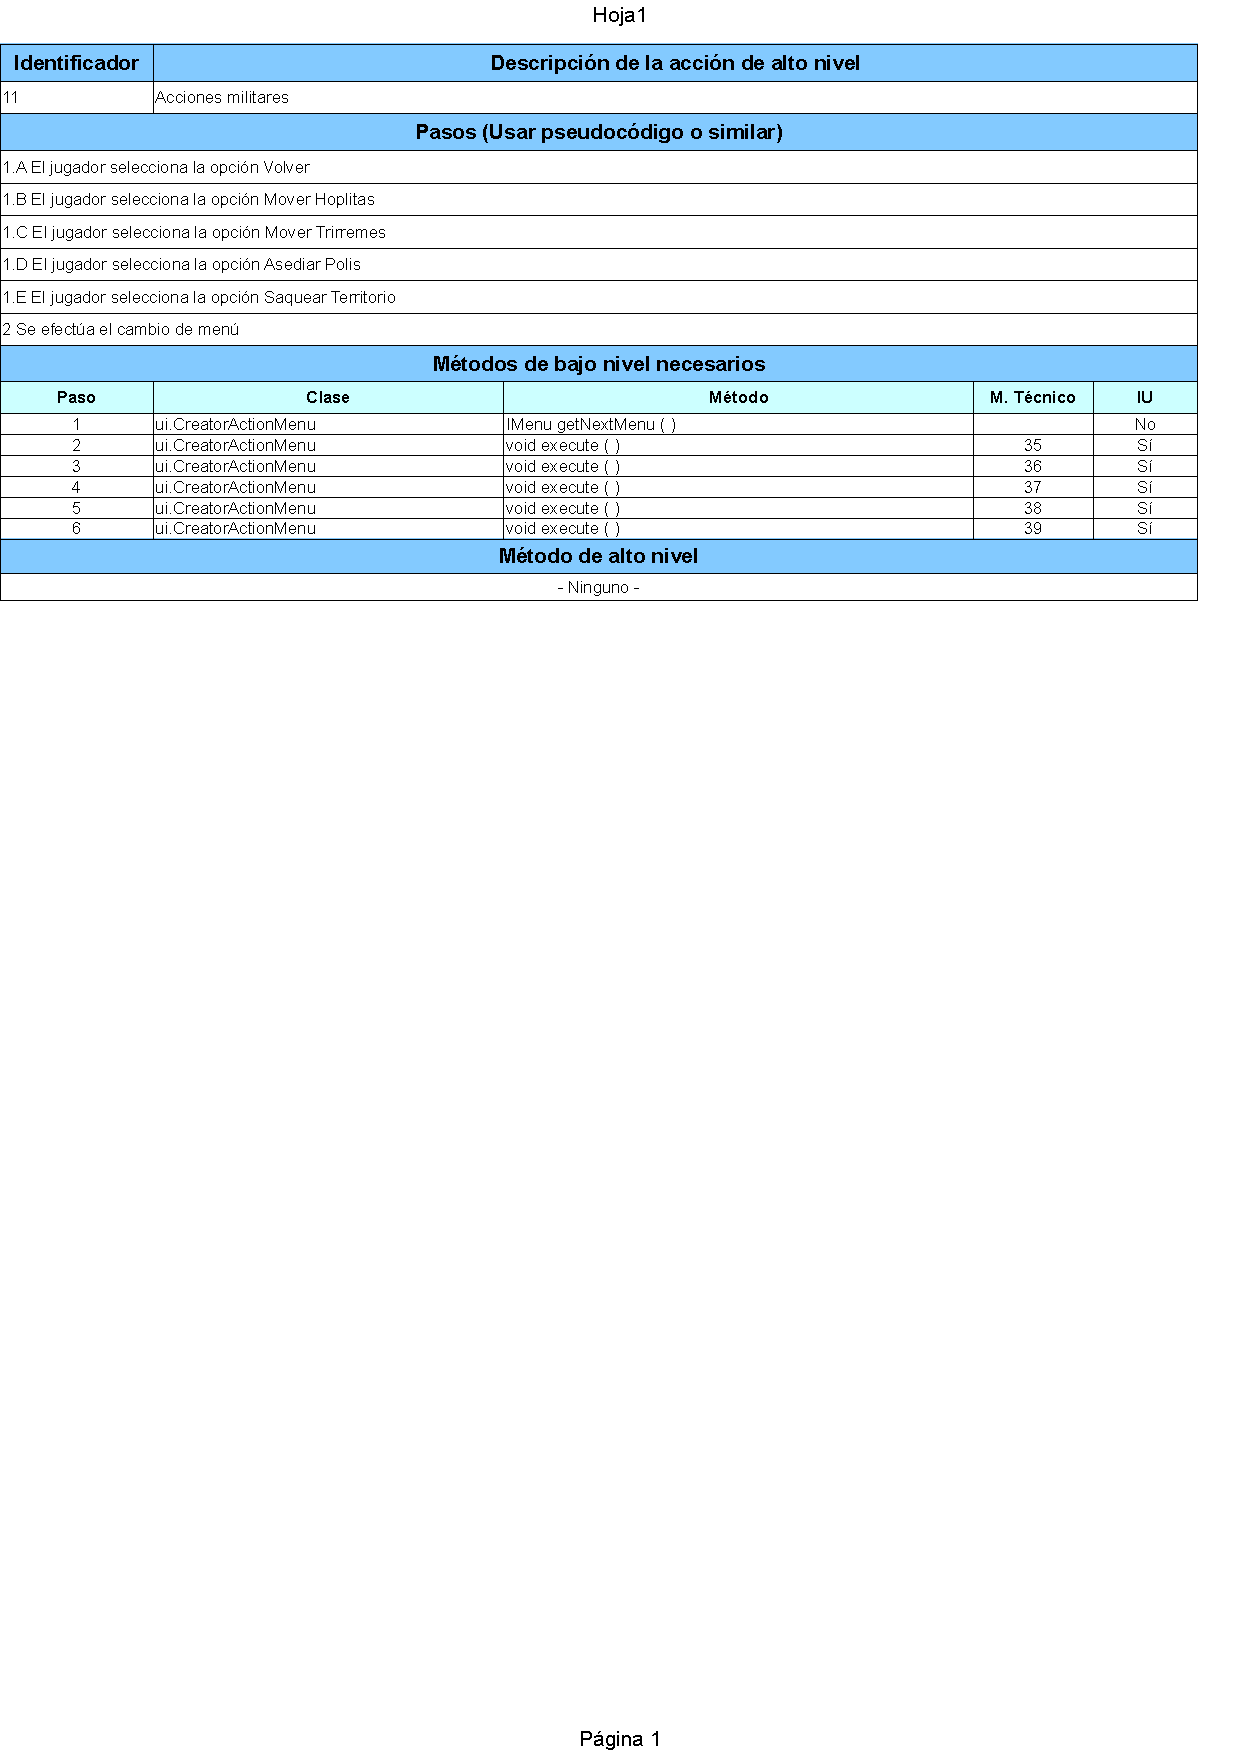
\includepdf[pages=-]{responsabilities-allocation/iteration7/IT7-11.pdf}
		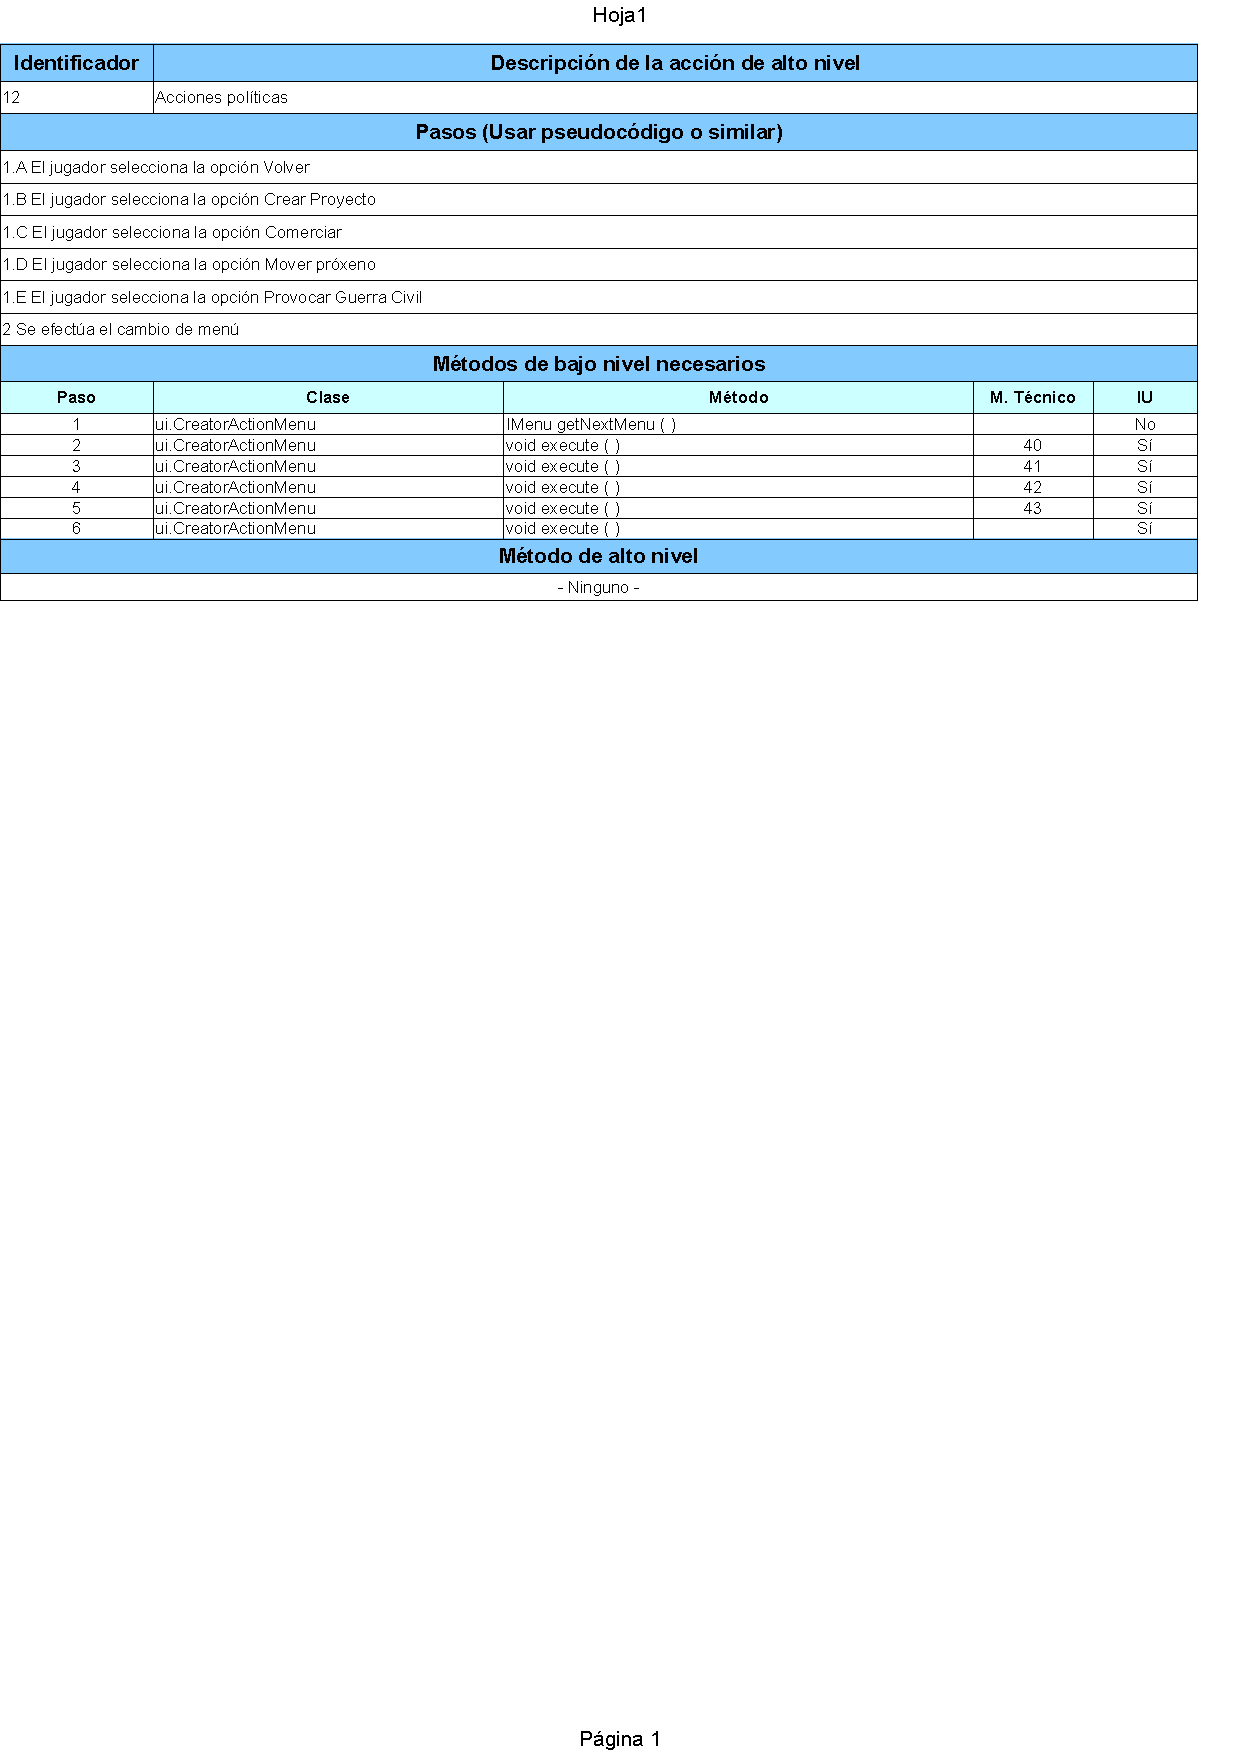
\includepdf[pages=-]{responsabilities-allocation/iteration7/IT7-12.pdf}
		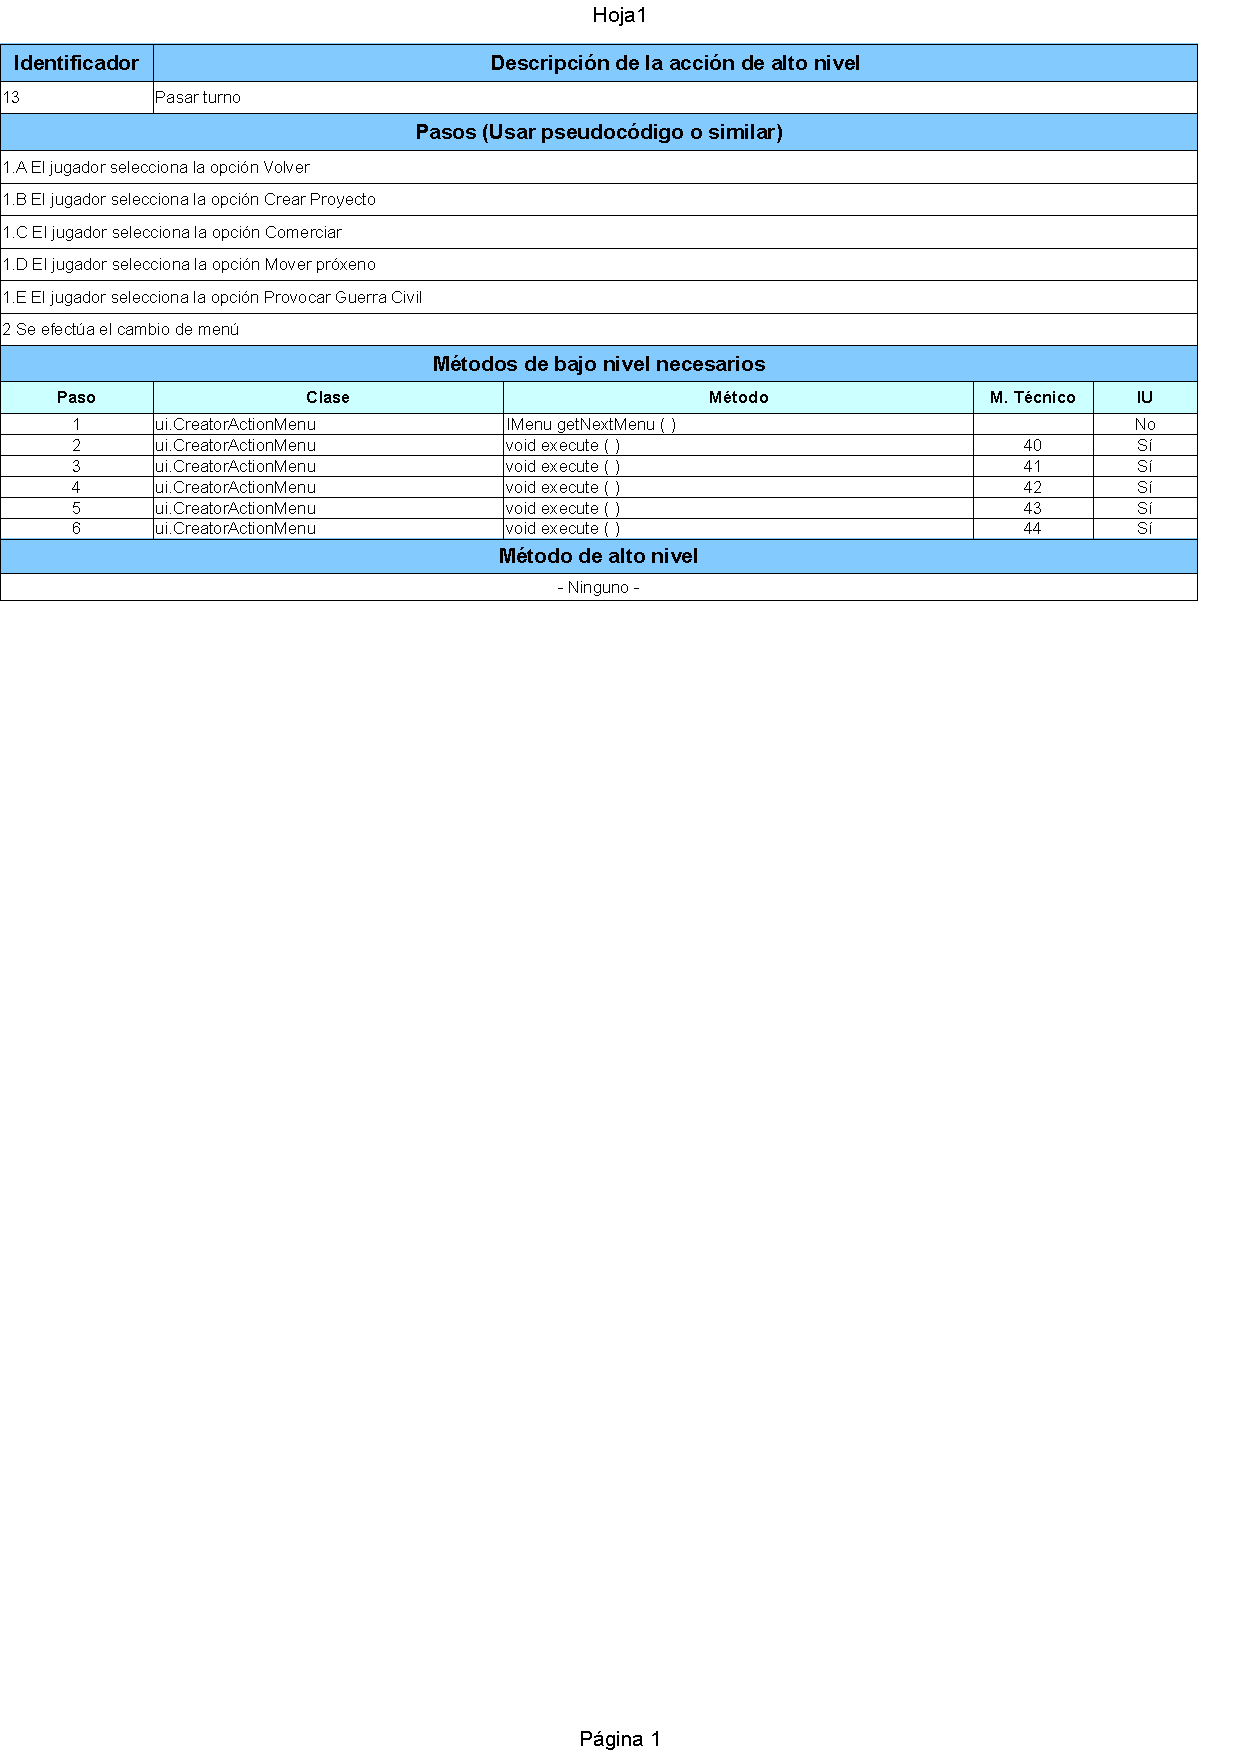
\includepdf[pages=-]{responsabilities-allocation/iteration7/IT7-13.pdf}
		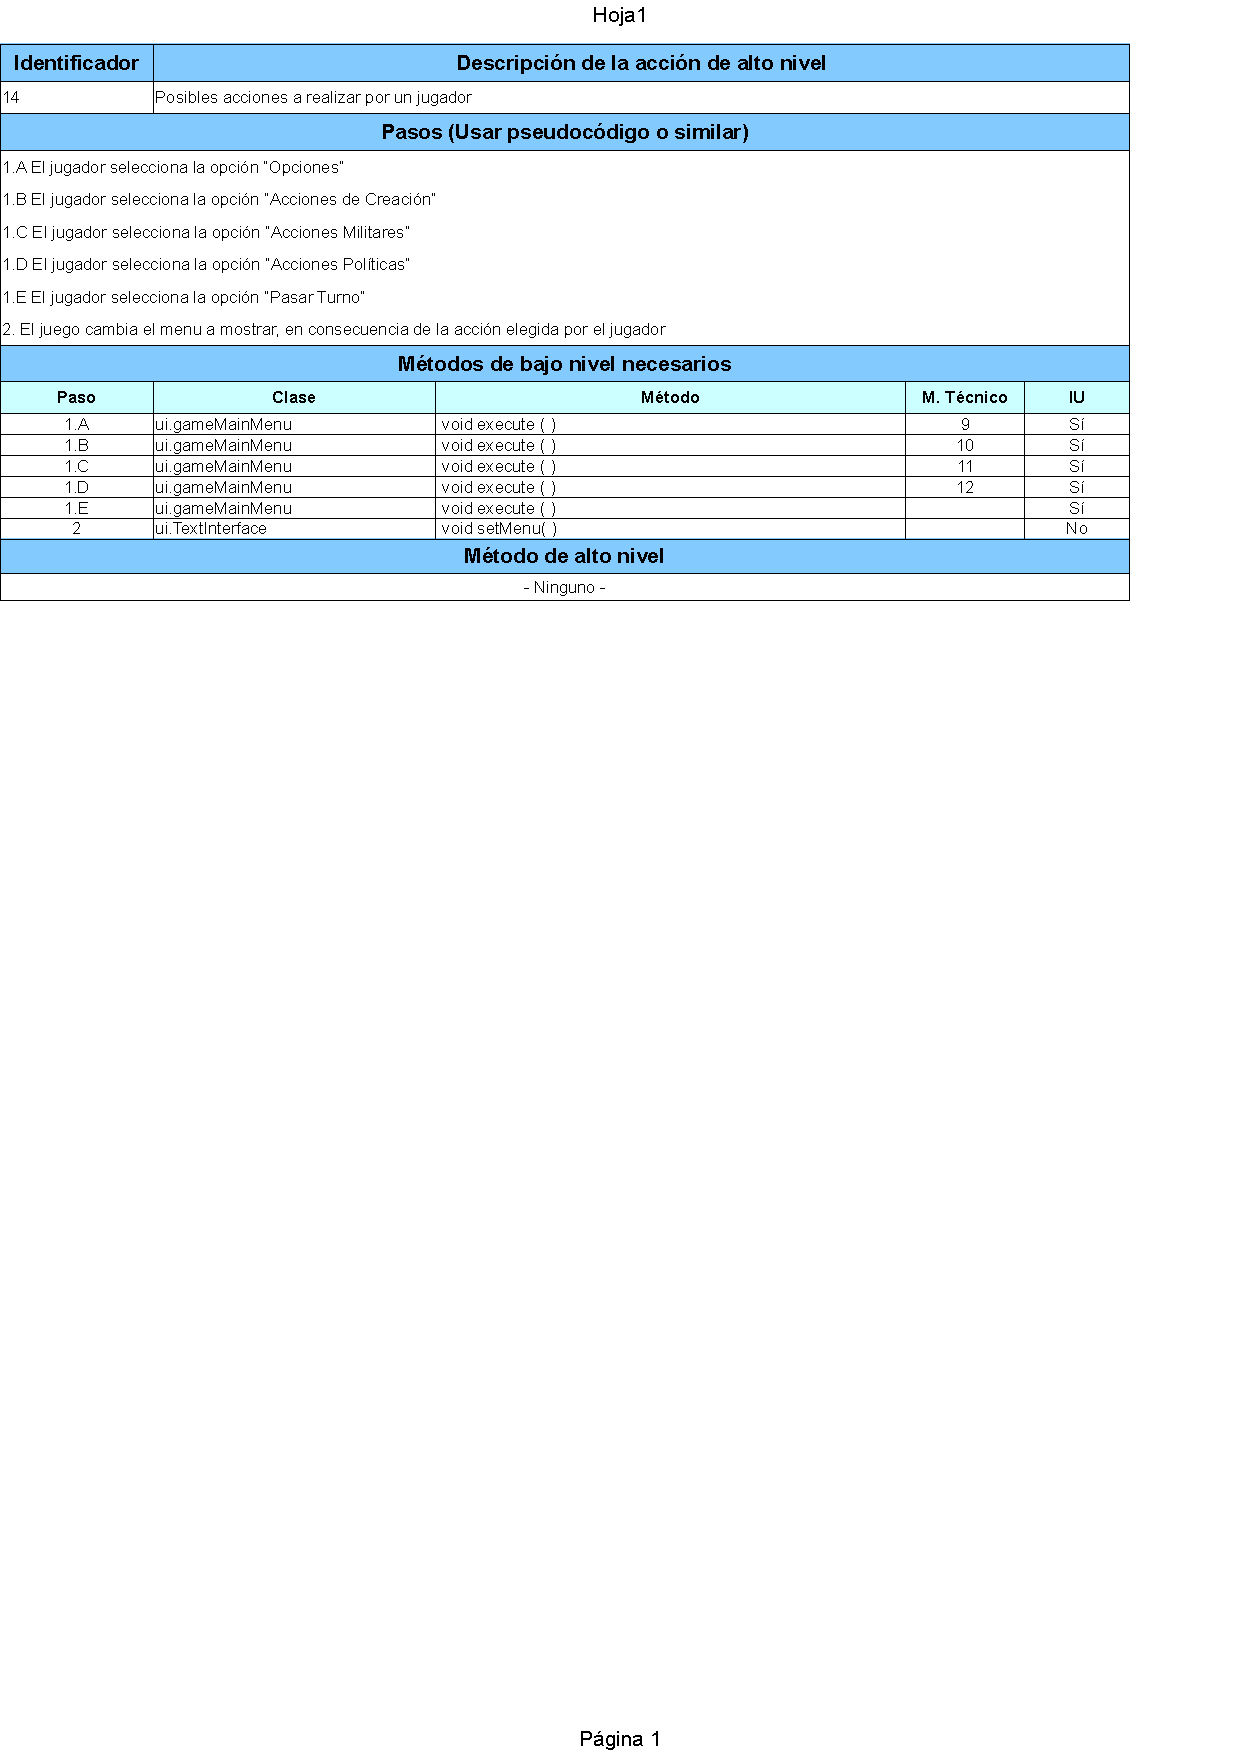
\includepdf[pages=-]{responsabilities-allocation/iteration7/IT7-14.pdf}
		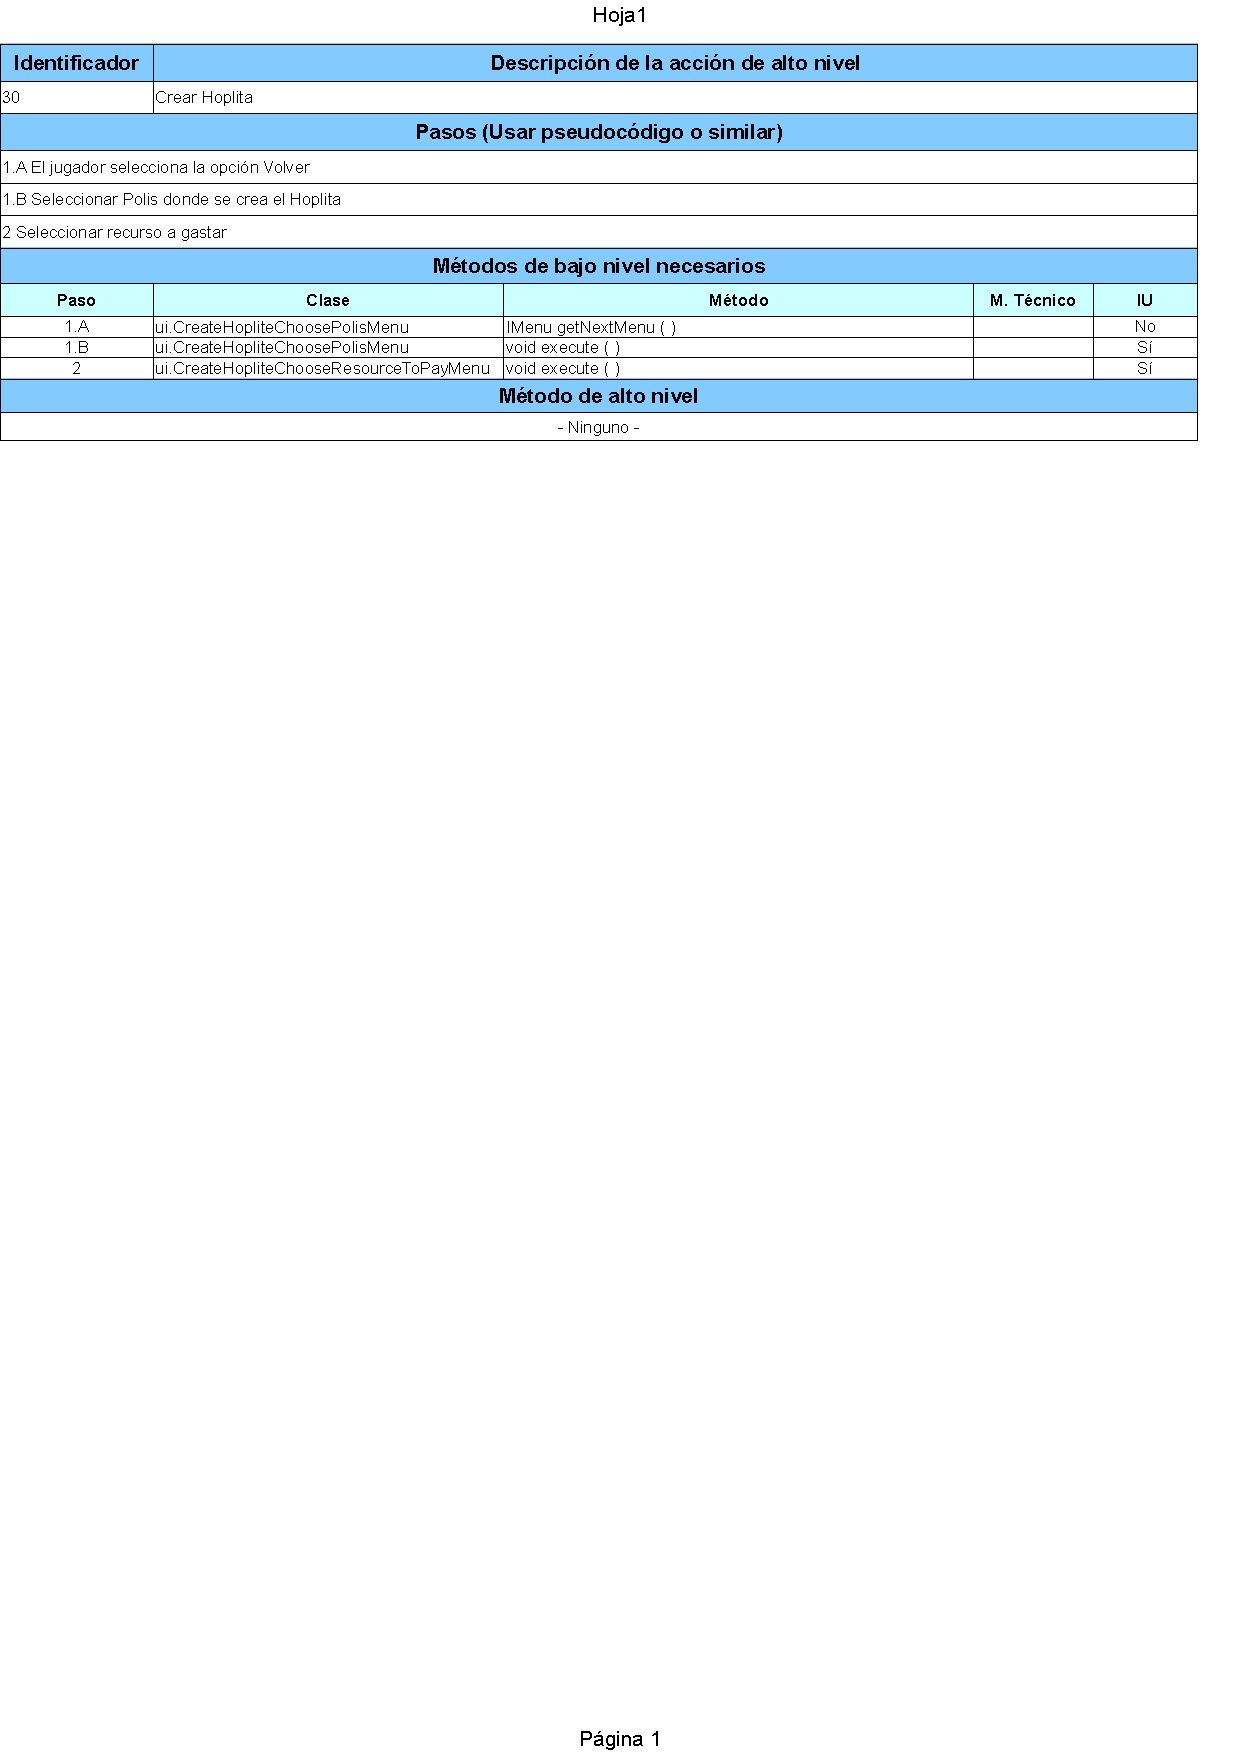
\includepdf[pages=-]{responsabilities-allocation/iteration7/IT7-30.pdf}
		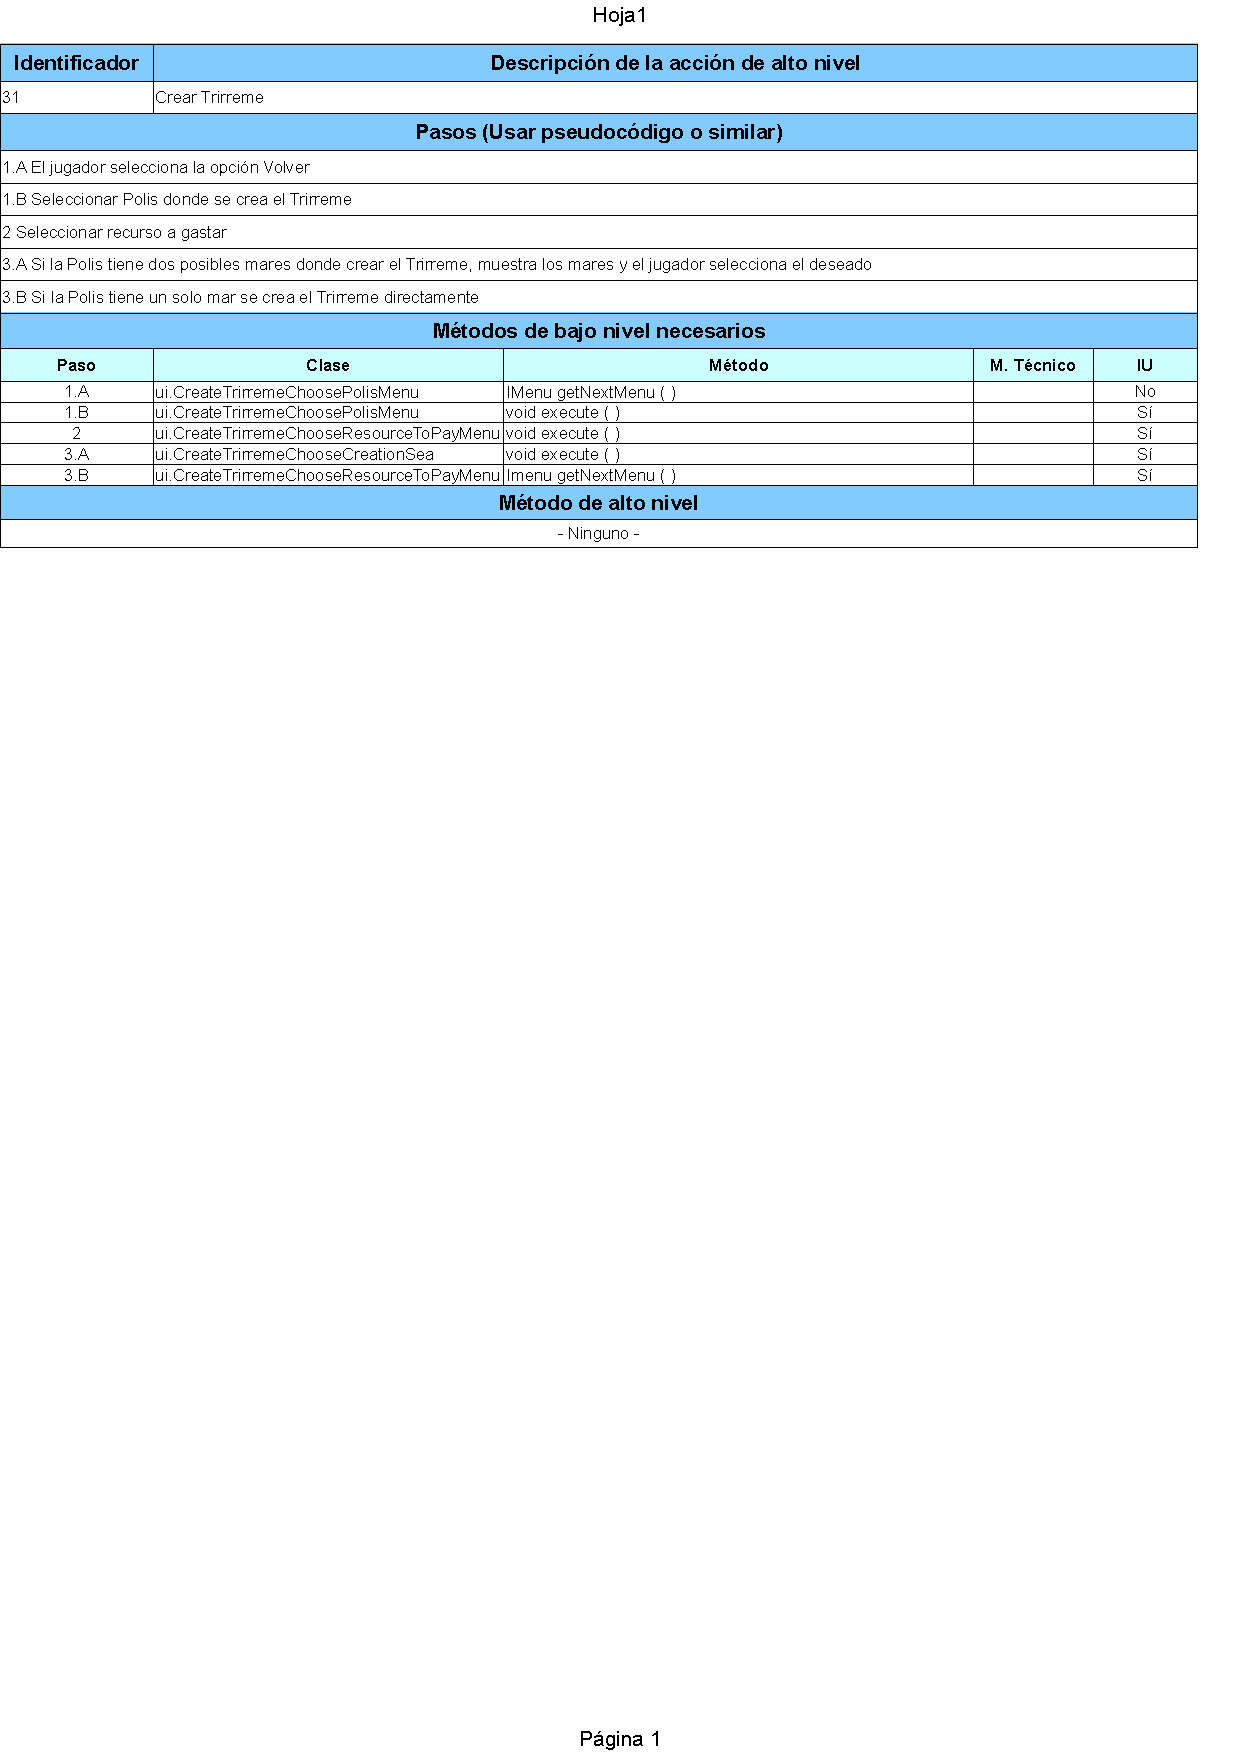
\includepdf[pages=-]{responsabilities-allocation/iteration7/IT7-31.pdf}
		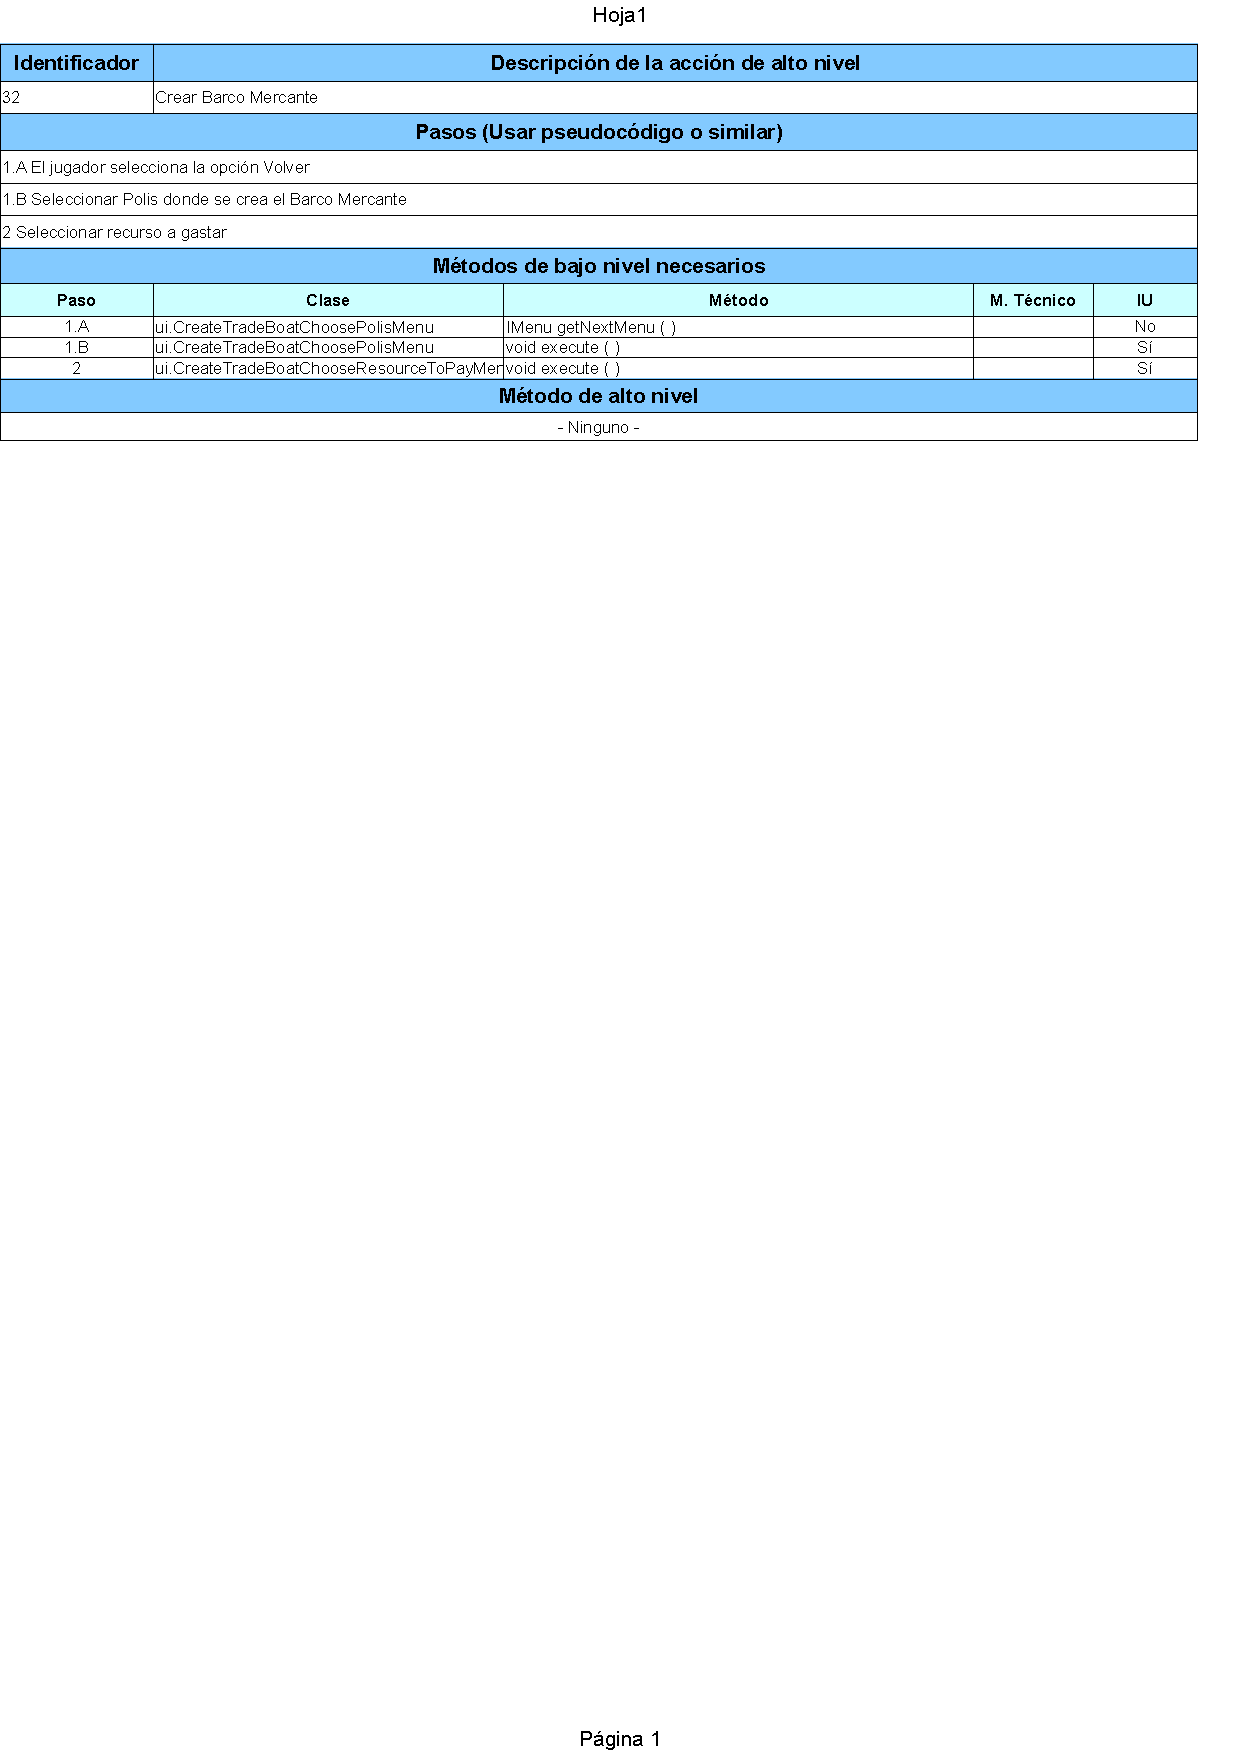
\includepdf[pages=-]{responsabilities-allocation/iteration7/IT7-32.pdf}
		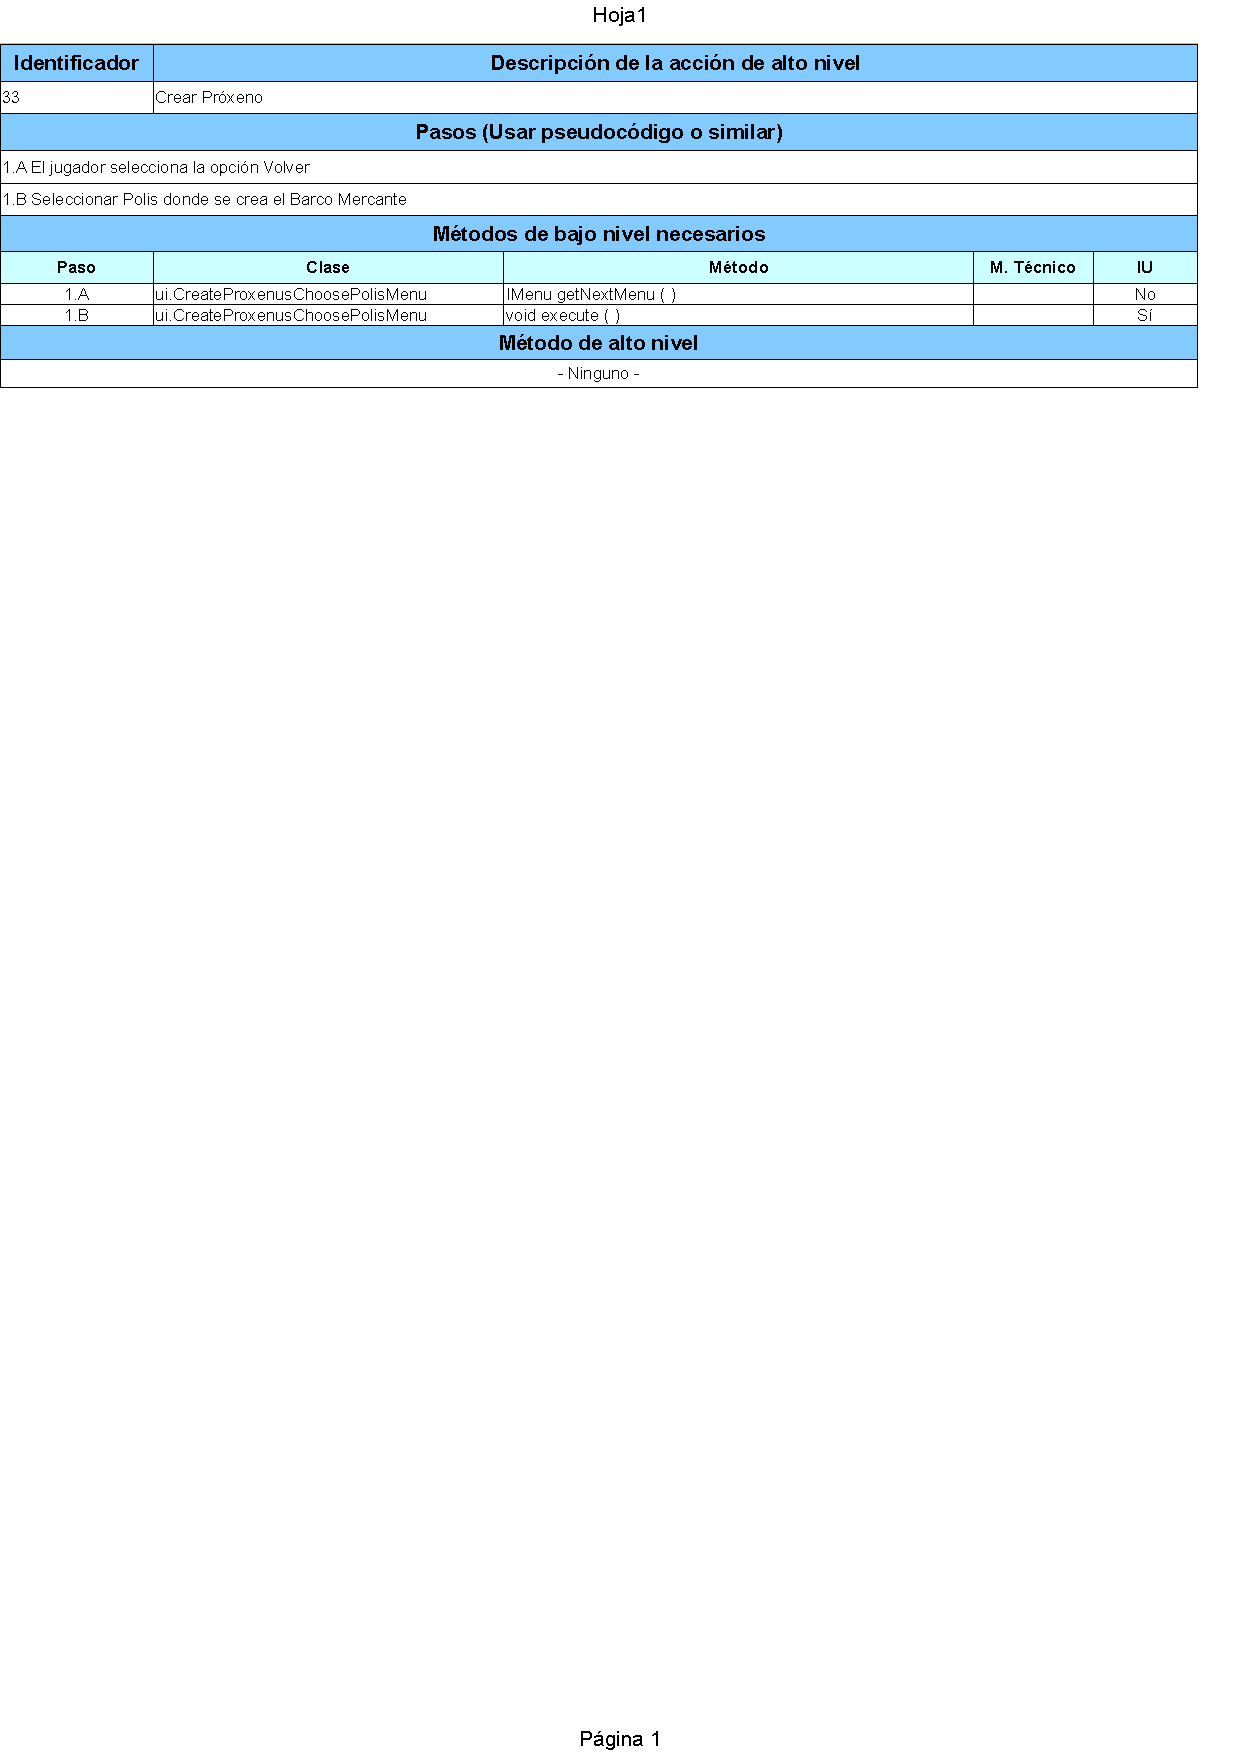
\includepdf[pages=-]{responsabilities-allocation/iteration7/IT7-33.pdf}
		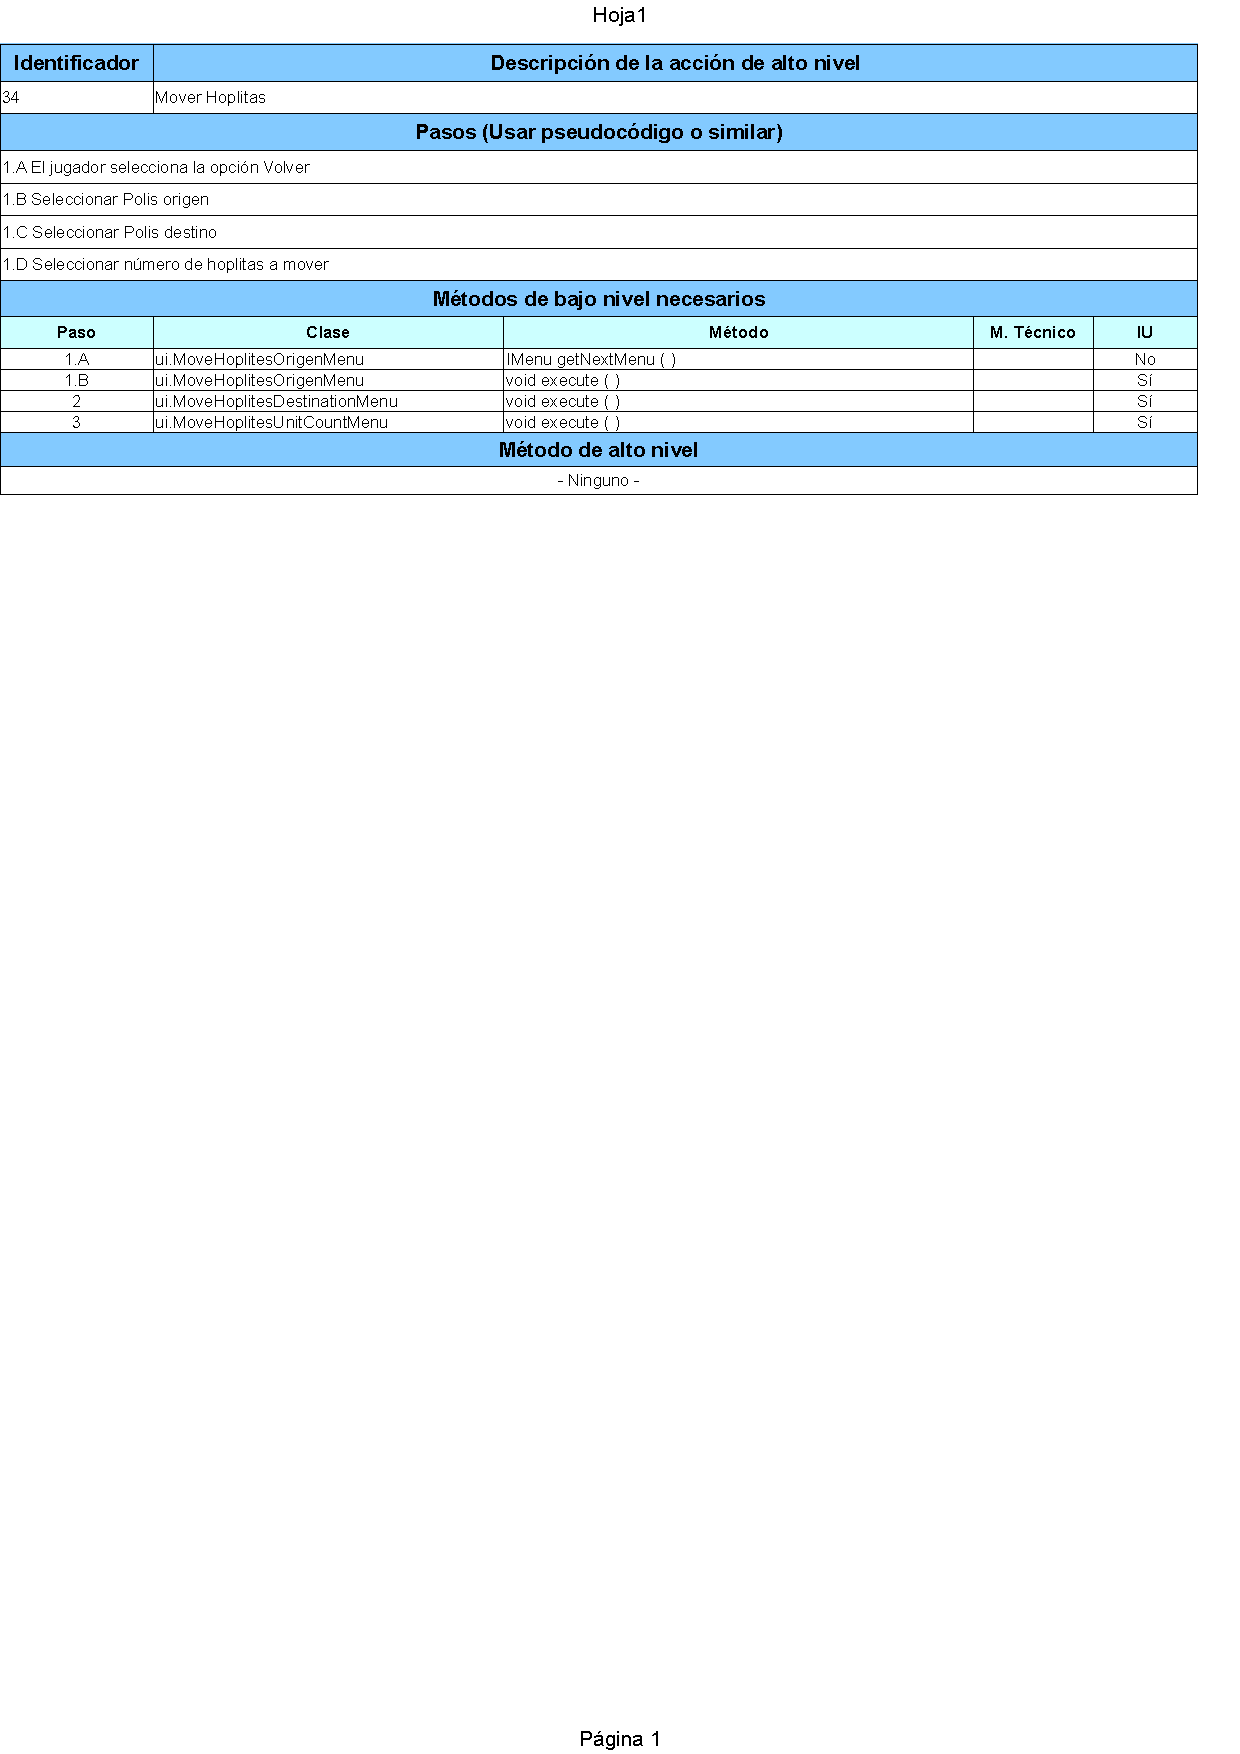
\includepdf[pages=-]{responsabilities-allocation/iteration7/IT7-34.pdf}
		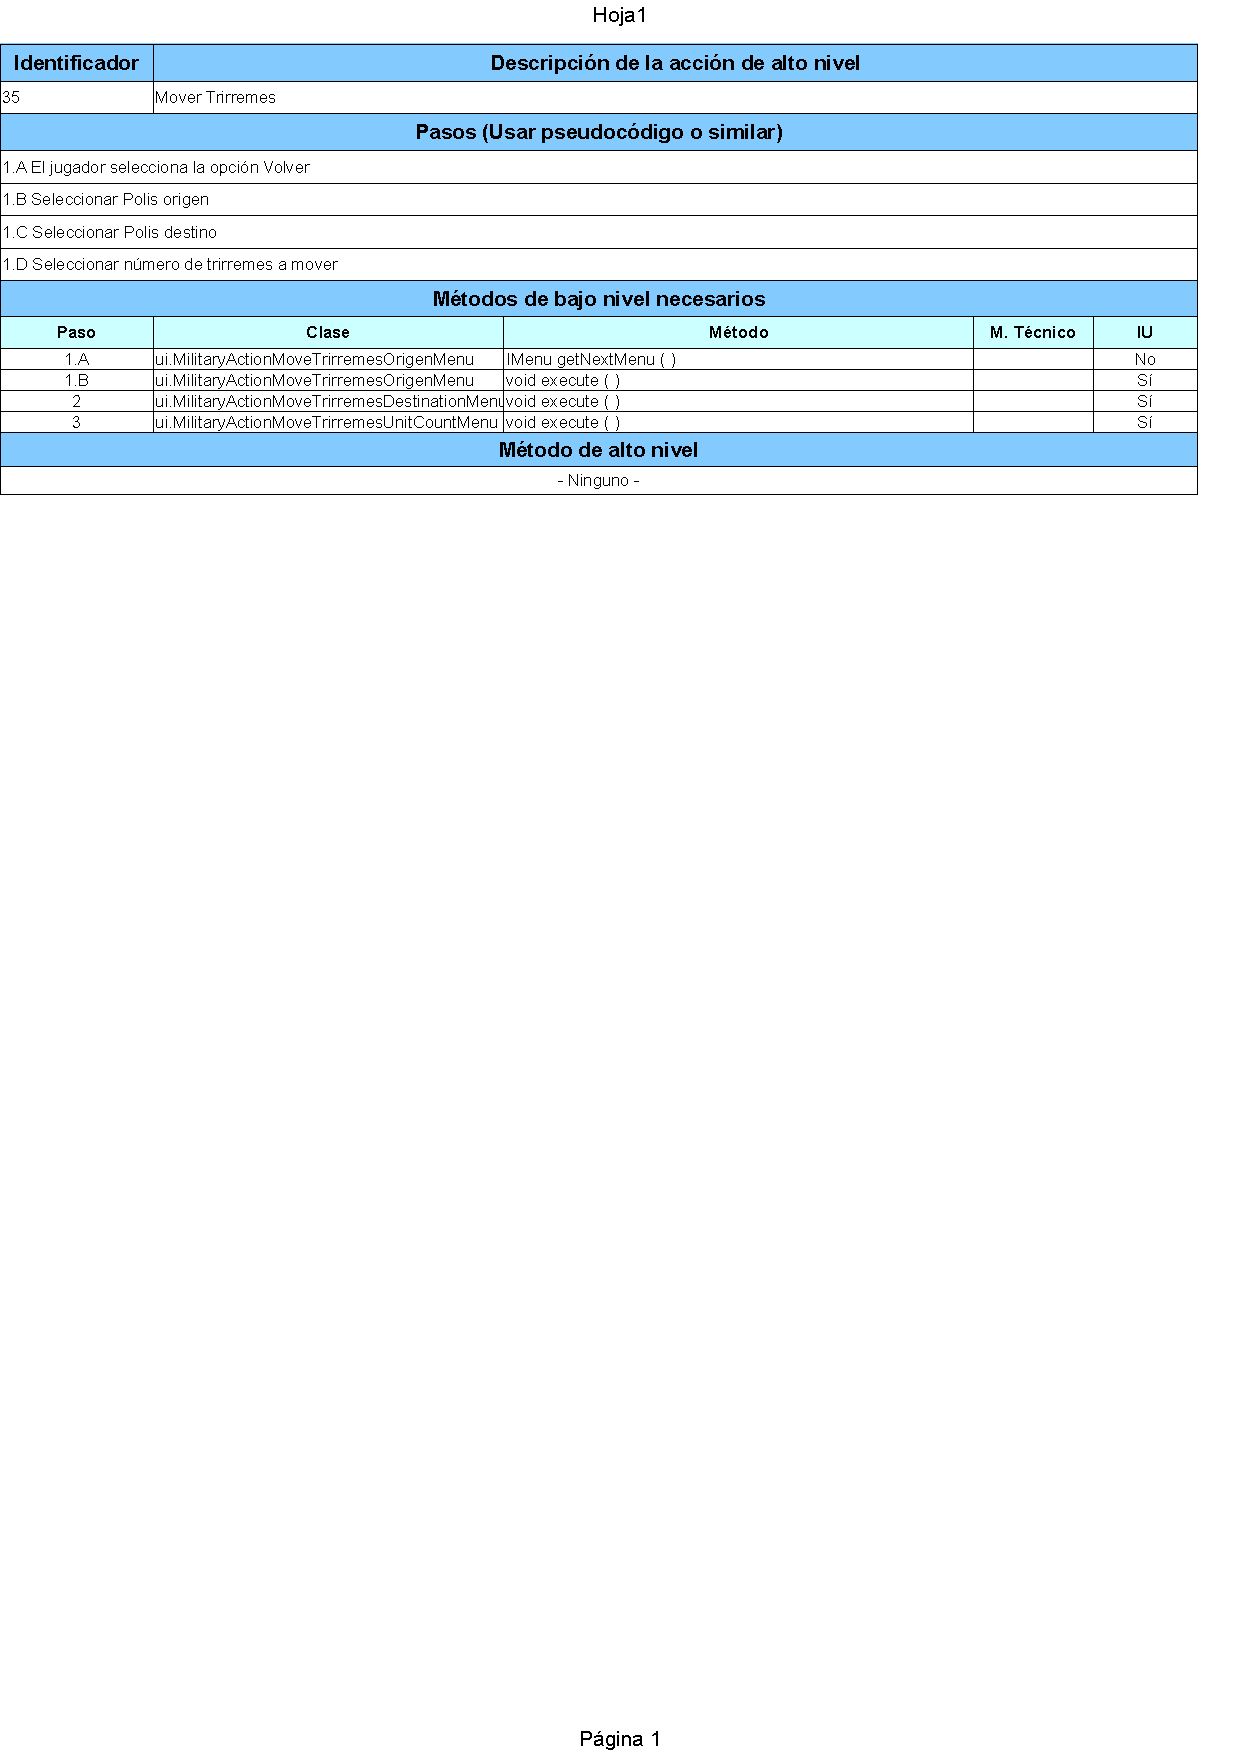
\includepdf[pages=-]{responsabilities-allocation/iteration7/IT7-35.pdf}
		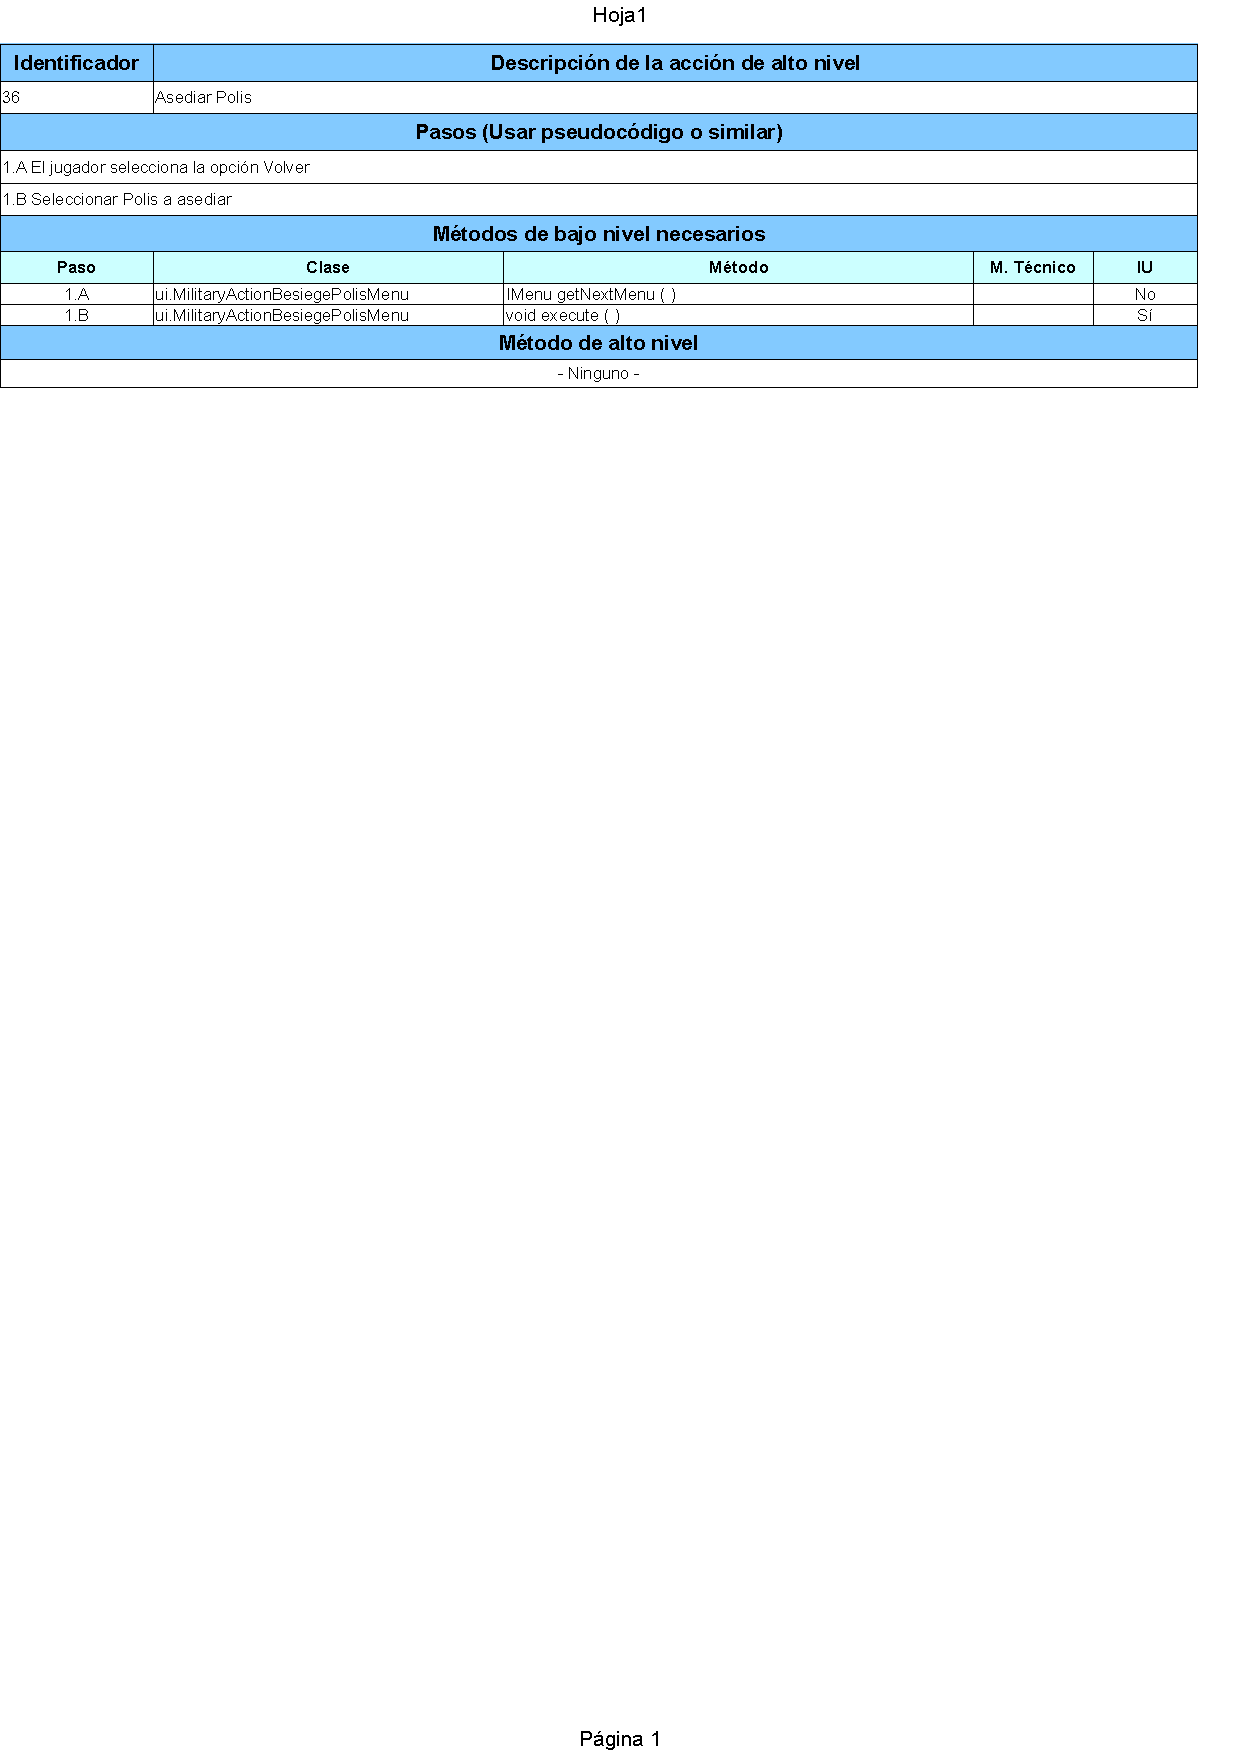
\includepdf[pages=-]{responsabilities-allocation/iteration7/IT7-36.pdf}
		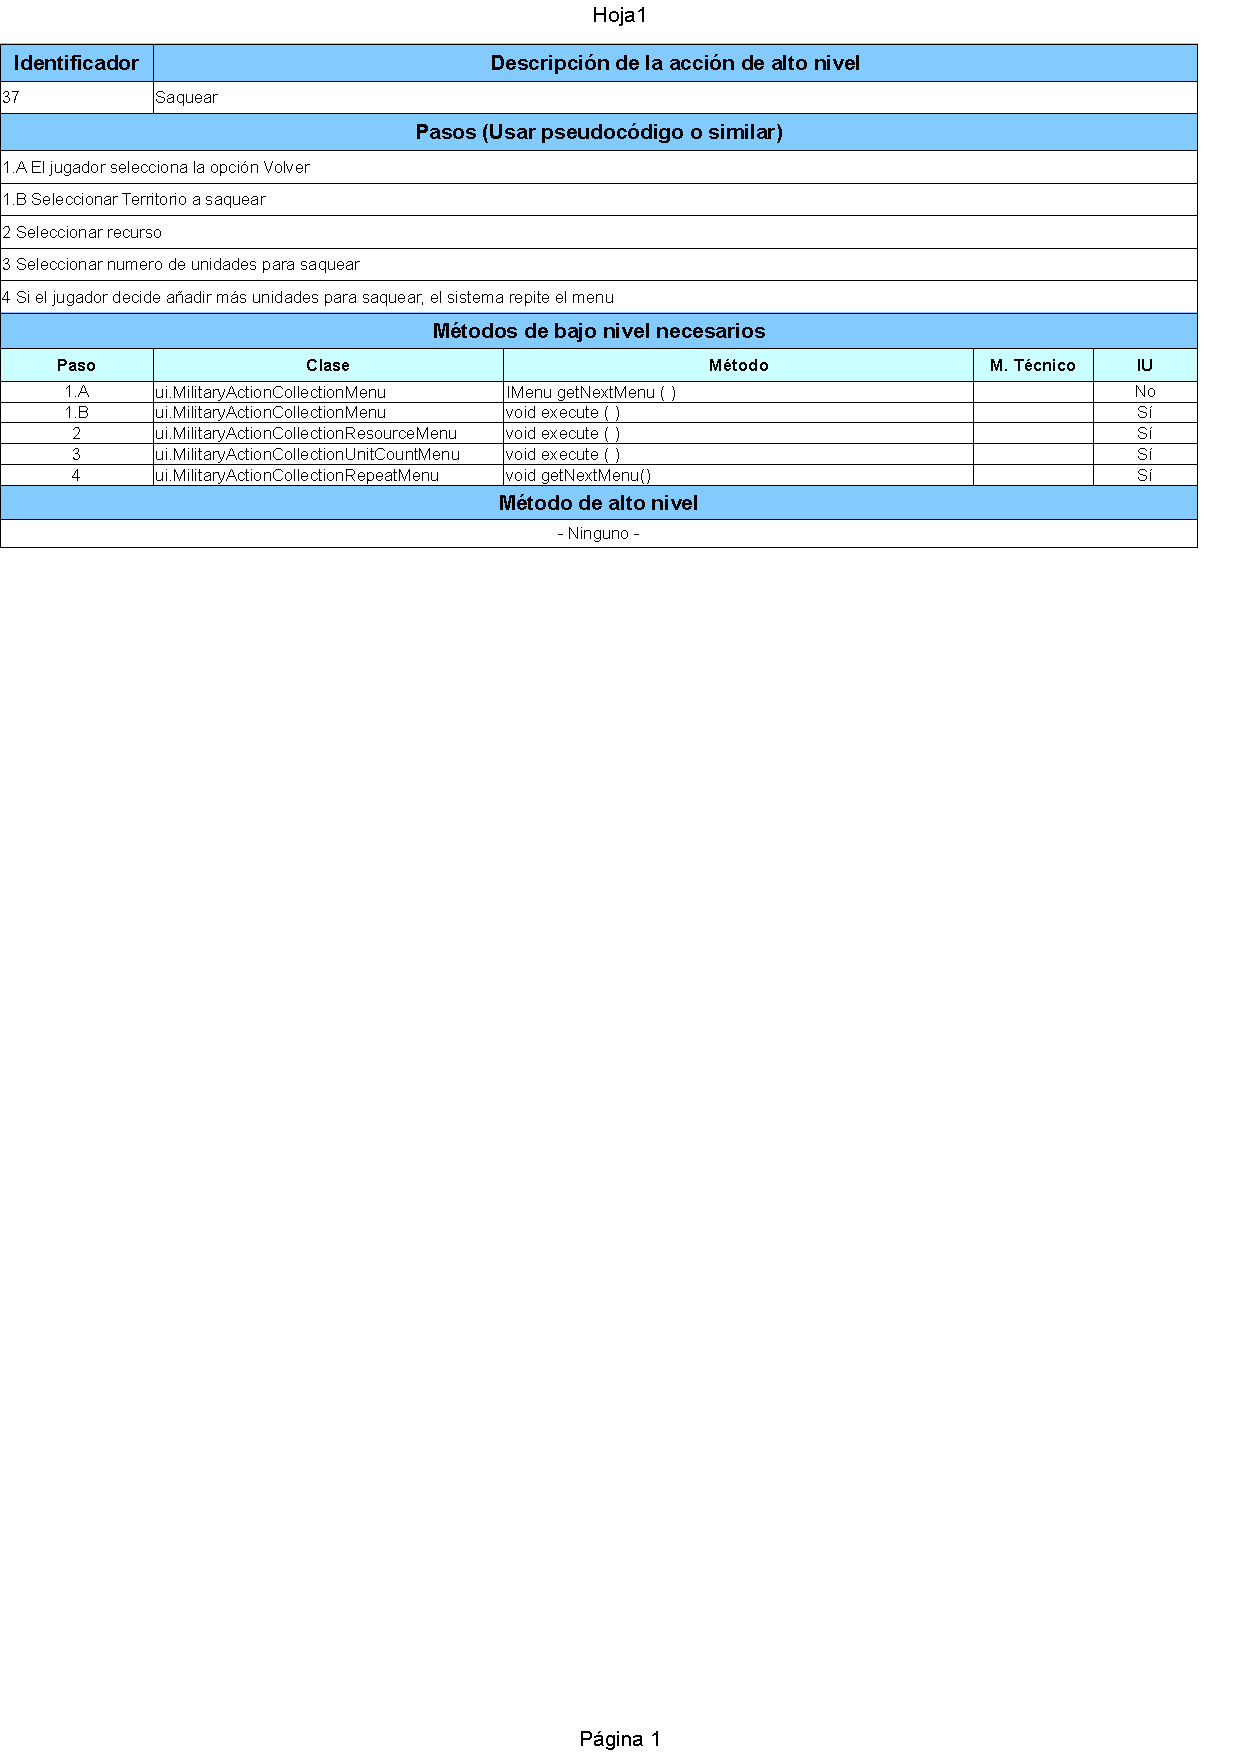
\includepdf[pages=-]{responsabilities-allocation/iteration7/IT7-37.pdf}
		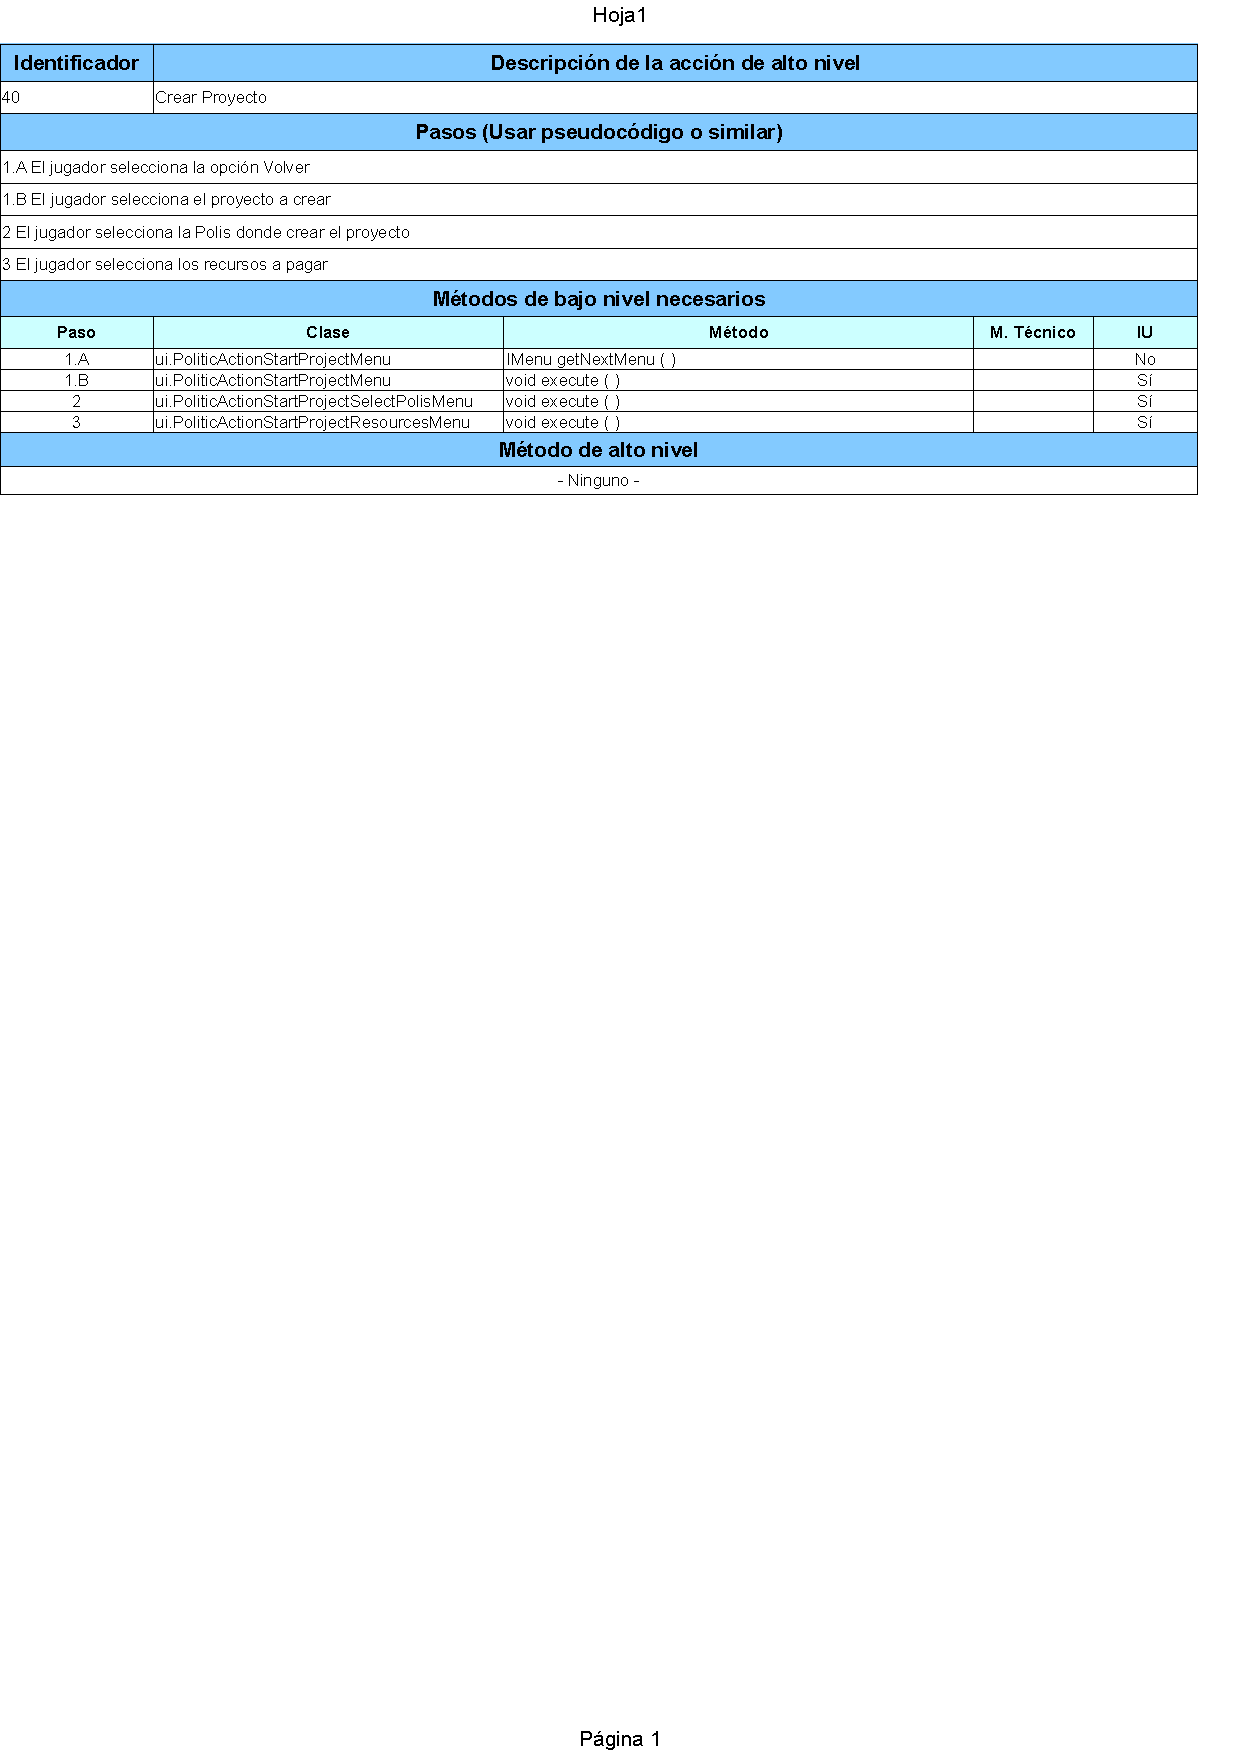
\includepdf[pages=-]{responsabilities-allocation/iteration7/IT7-40.pdf}
		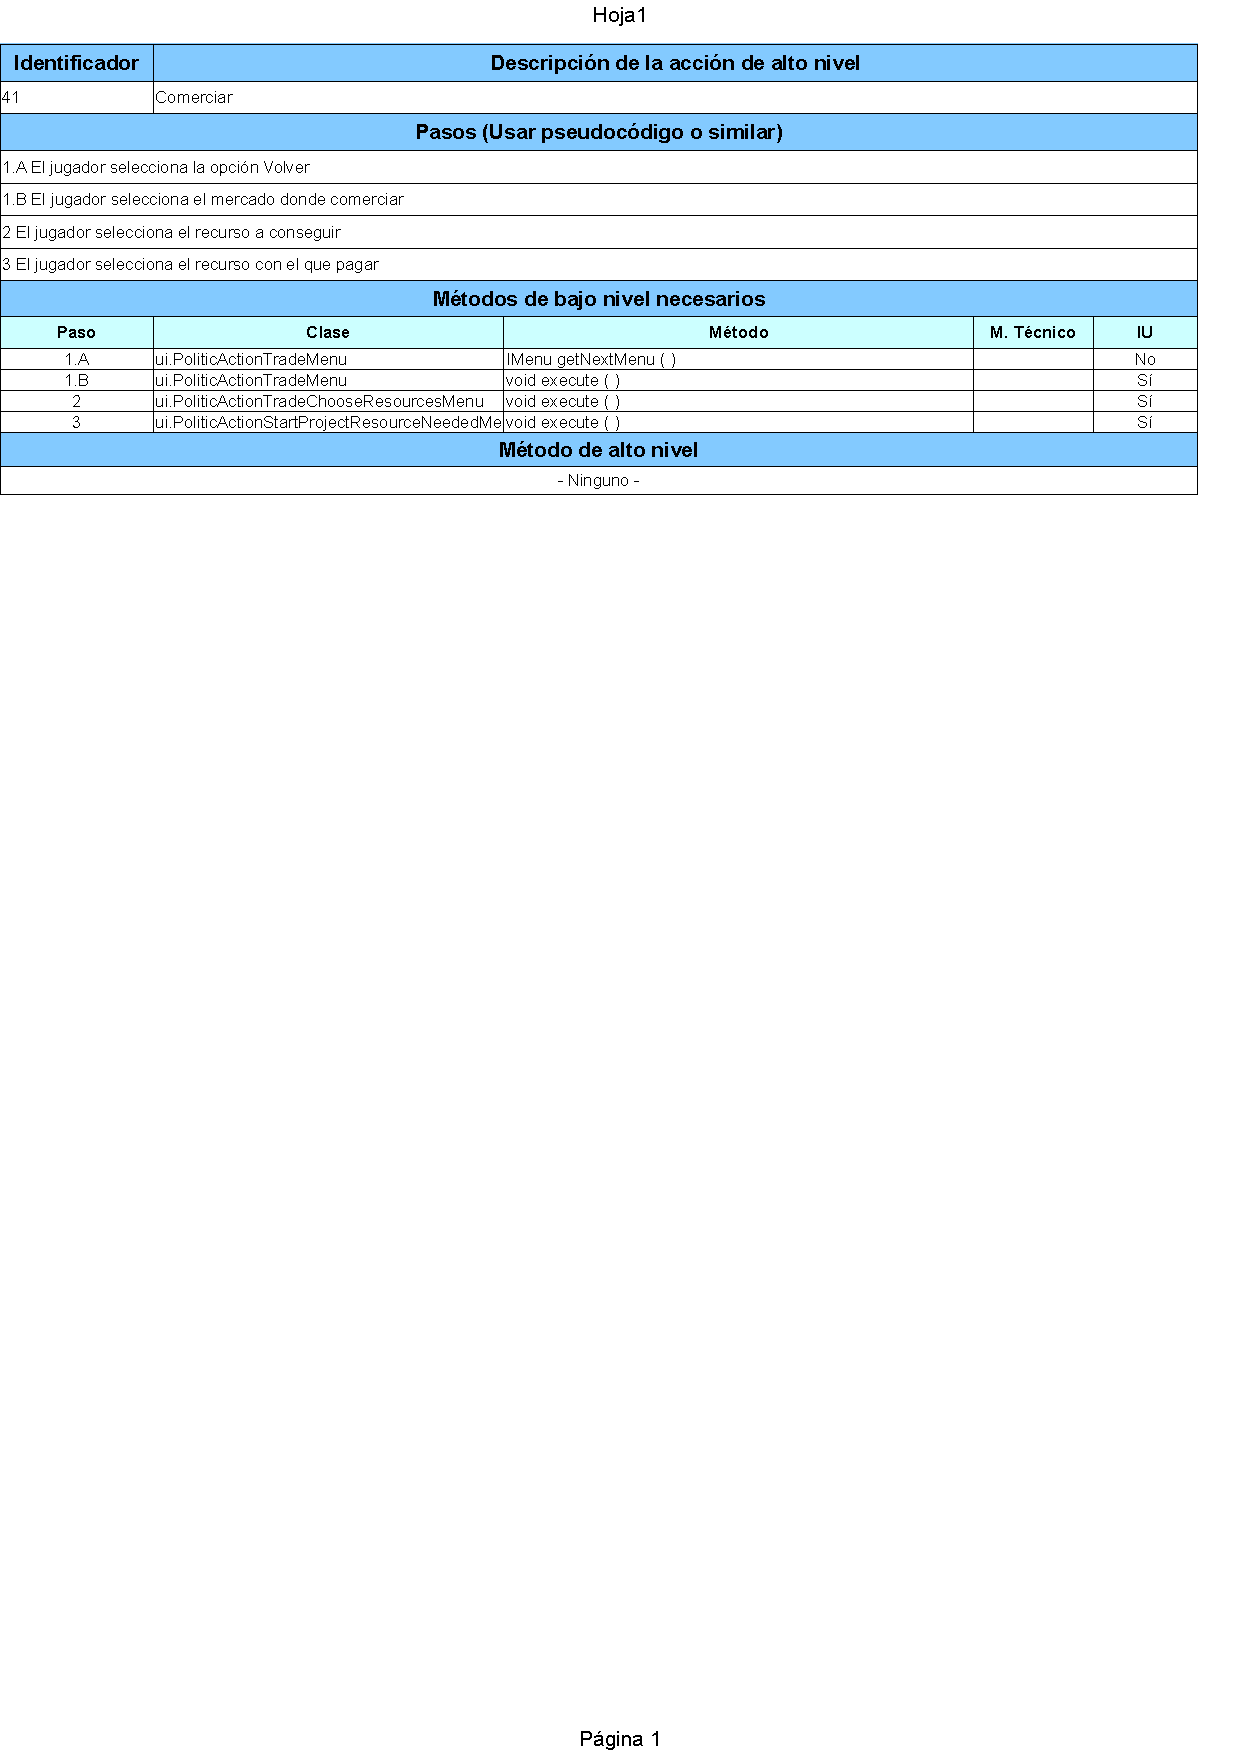
\includepdf[pages=-]{responsabilities-allocation/iteration7/IT7-41.pdf}
		\includepdf[pages=-]{responsabilities-allocation/iteration7/IT7-42.pdf}
		\includepdf[pages=-]{responsabilities-allocation/iteration7/IT7-43.pdf}
		
	\section{Memorando técnico}
		\includepdf[pages=-]{memorandos/iteration7/memorandos.pdf}
		
	\section{Seguimiento}
		\begin{tabular}{|c|c|c|c|}
			\hline
			Nombre & Tiempo dedicado acumulado & Puntuación & Puntuación acumulada\\
			\hline
			Samuel Navas Portillo & 126 & 1 & 39\\
			Juan Jesús Pérez Luna & 136h 30min & 1 & 39\\
			Manuel de los Santos Campos & 69 & 9 & 35\\
			María José Sancha Maya & 48h 30min & 9 & 28\\
			Ángel Martínez Olivares & 59h 30min & 9 & 33\\
			José Antonio Jiménez Carmona & 82 & 1 & 36\\
			\hline
		\end{tabular}
\end{document}
